\chapter{Development of a Muon Identification acquisition and reconstruction framework for ALICE RUN3}

\section{Motivation}
% By 2021 ALICE will undergo a major upgrade concerning the luminosity achievable in Pb-Pb collisions.
The second phase of data taking, called Run 2, will be over by the end of 2018. 
After that, the LHC will stop for two years (long shutdown), during which an upgrade that will increase the luminosity reach in $Pb-Pb$ from $\approx 1\ Hz/mb$ (corresponding to a hadronic interaction rate of $\approx8\ kHz$) to $\approx6\ Hz/mb (\approx50\ kHz)$ will be performed.
At the same time, ALICE will undergo a major upgrade of detectors, electronics and readout that will allow the experiment to cope with the increased Pb-Pb interaction rate, and to also take pp interactions up to $\approx1\ MHz$ (vs the current $\approx100 kHz$) \cite{Abelev:1625842, CERN-LHCC-2013-020, CERN-LHCC-2015-001, Antonioli:1603472, Buncic:2011297}.
% After the Long Shutdown 2 (LS2 from now on) the delivered instantaneous luminosity will reach $6\cdot10^{27} cm^{-2}s^{-1}$ in Pb-Pb collisions, feeding the ALICE detectors with up to 50 kHz of minimum bias collision rate in Pb-Pb and 200 kHz in pp.

% The $O^2$ project follows the upgrade of the LHC triggered by the increase of statistics necessary for new and improved measurements.
A requirement of a total integrated luminosity of $13\ nb^{-1}$ in Pb-Pb collisions was formulated with the ALICE Letter Of Intent (LOI) \cite{ALICE_LOI}, split in $10\ nb^{-1}$ at nominal solenoid magnetic field and $3\ nb^{-1}$ at a reduced field of $0.2\ T$.
These requirements are related to specific performance figures, concerning open heavy flavours, low mass dileptons and quarkonium measurements.
In particular the plans for $J/\psi$ ($\psi(\mathrm{2S})$) foresee to know its $R_{\mathrm{AA}}$ down to $p_{\mathrm{T}} = 0$ with statistical precision higher than $1\%$ ($10\%$) over the whole rapidity interval and its elliptic flow, quantified through the $\nu_2$ coefficient \cite{Acharya:2017tgv}, down to $p_{\mathrm{T}} = 0$ with an absolute precision of $0.05$.

Some of the physics topics addressed by ALICE concern physics probes characterized by very small signal-to-background ratios.
In order to obtain significant measurements it is important to collect very large statistics.
The upgrade of the LHC builds up in this direction.
The foreseen increase of the luminosity provided by the LHC will cause an increase of collected data rate.
The upgrade of the electronics will allow one to increase the data to a value of about two orders of magnitude larger than the one that ALICE experienced during LHC RUN1 and RUN2.
In addition to the technical difficulty of collecting high rate data avoiding bottlenecks, another challenge is represented by the way of triggering the acquisition of interesting events.
One of the main goals of the new data campaign is the study of rare probes down to low transverse momenta, a region where the large background makes the triggering techniques very inefficient or even impossible in many situations.
% Already in standard running conditions, the presence of a very large background makes standard triggering techniques very inefficient, and impossible in many situations.
Such increase of data size, combined with the high collision and acquisition rates, makes standard approaches difficult to apply without enormous (technical and economical) efforts for the upgrade of computing capabilities.
Since the required scaling of computing infrastructure cannot cope with the data throughput increase, a new acquisition and processing paradigm had to be developed.
The basic idea is to reduce the data size as early as possible in the stream that goes from the detector to the storage and reconstruction (Fig. \ref{fig:O2_sketch}).
This goal can be achieved adding pre-processing and reconstruction layers close to the detector acquisition logic.
For example some detectors will be equipped with a zero suppression algorithm to reduce the volume of data without losing useful information.
Such fast reconstruction will be performed synchronously with the data production and will be based on preliminary calibration and alignment information.
At this stage the detectors will operate as stand alone items and no merging of the data will be performed prior to the raw reconstruction.

\begin{figure}[!t]
\begin{center}
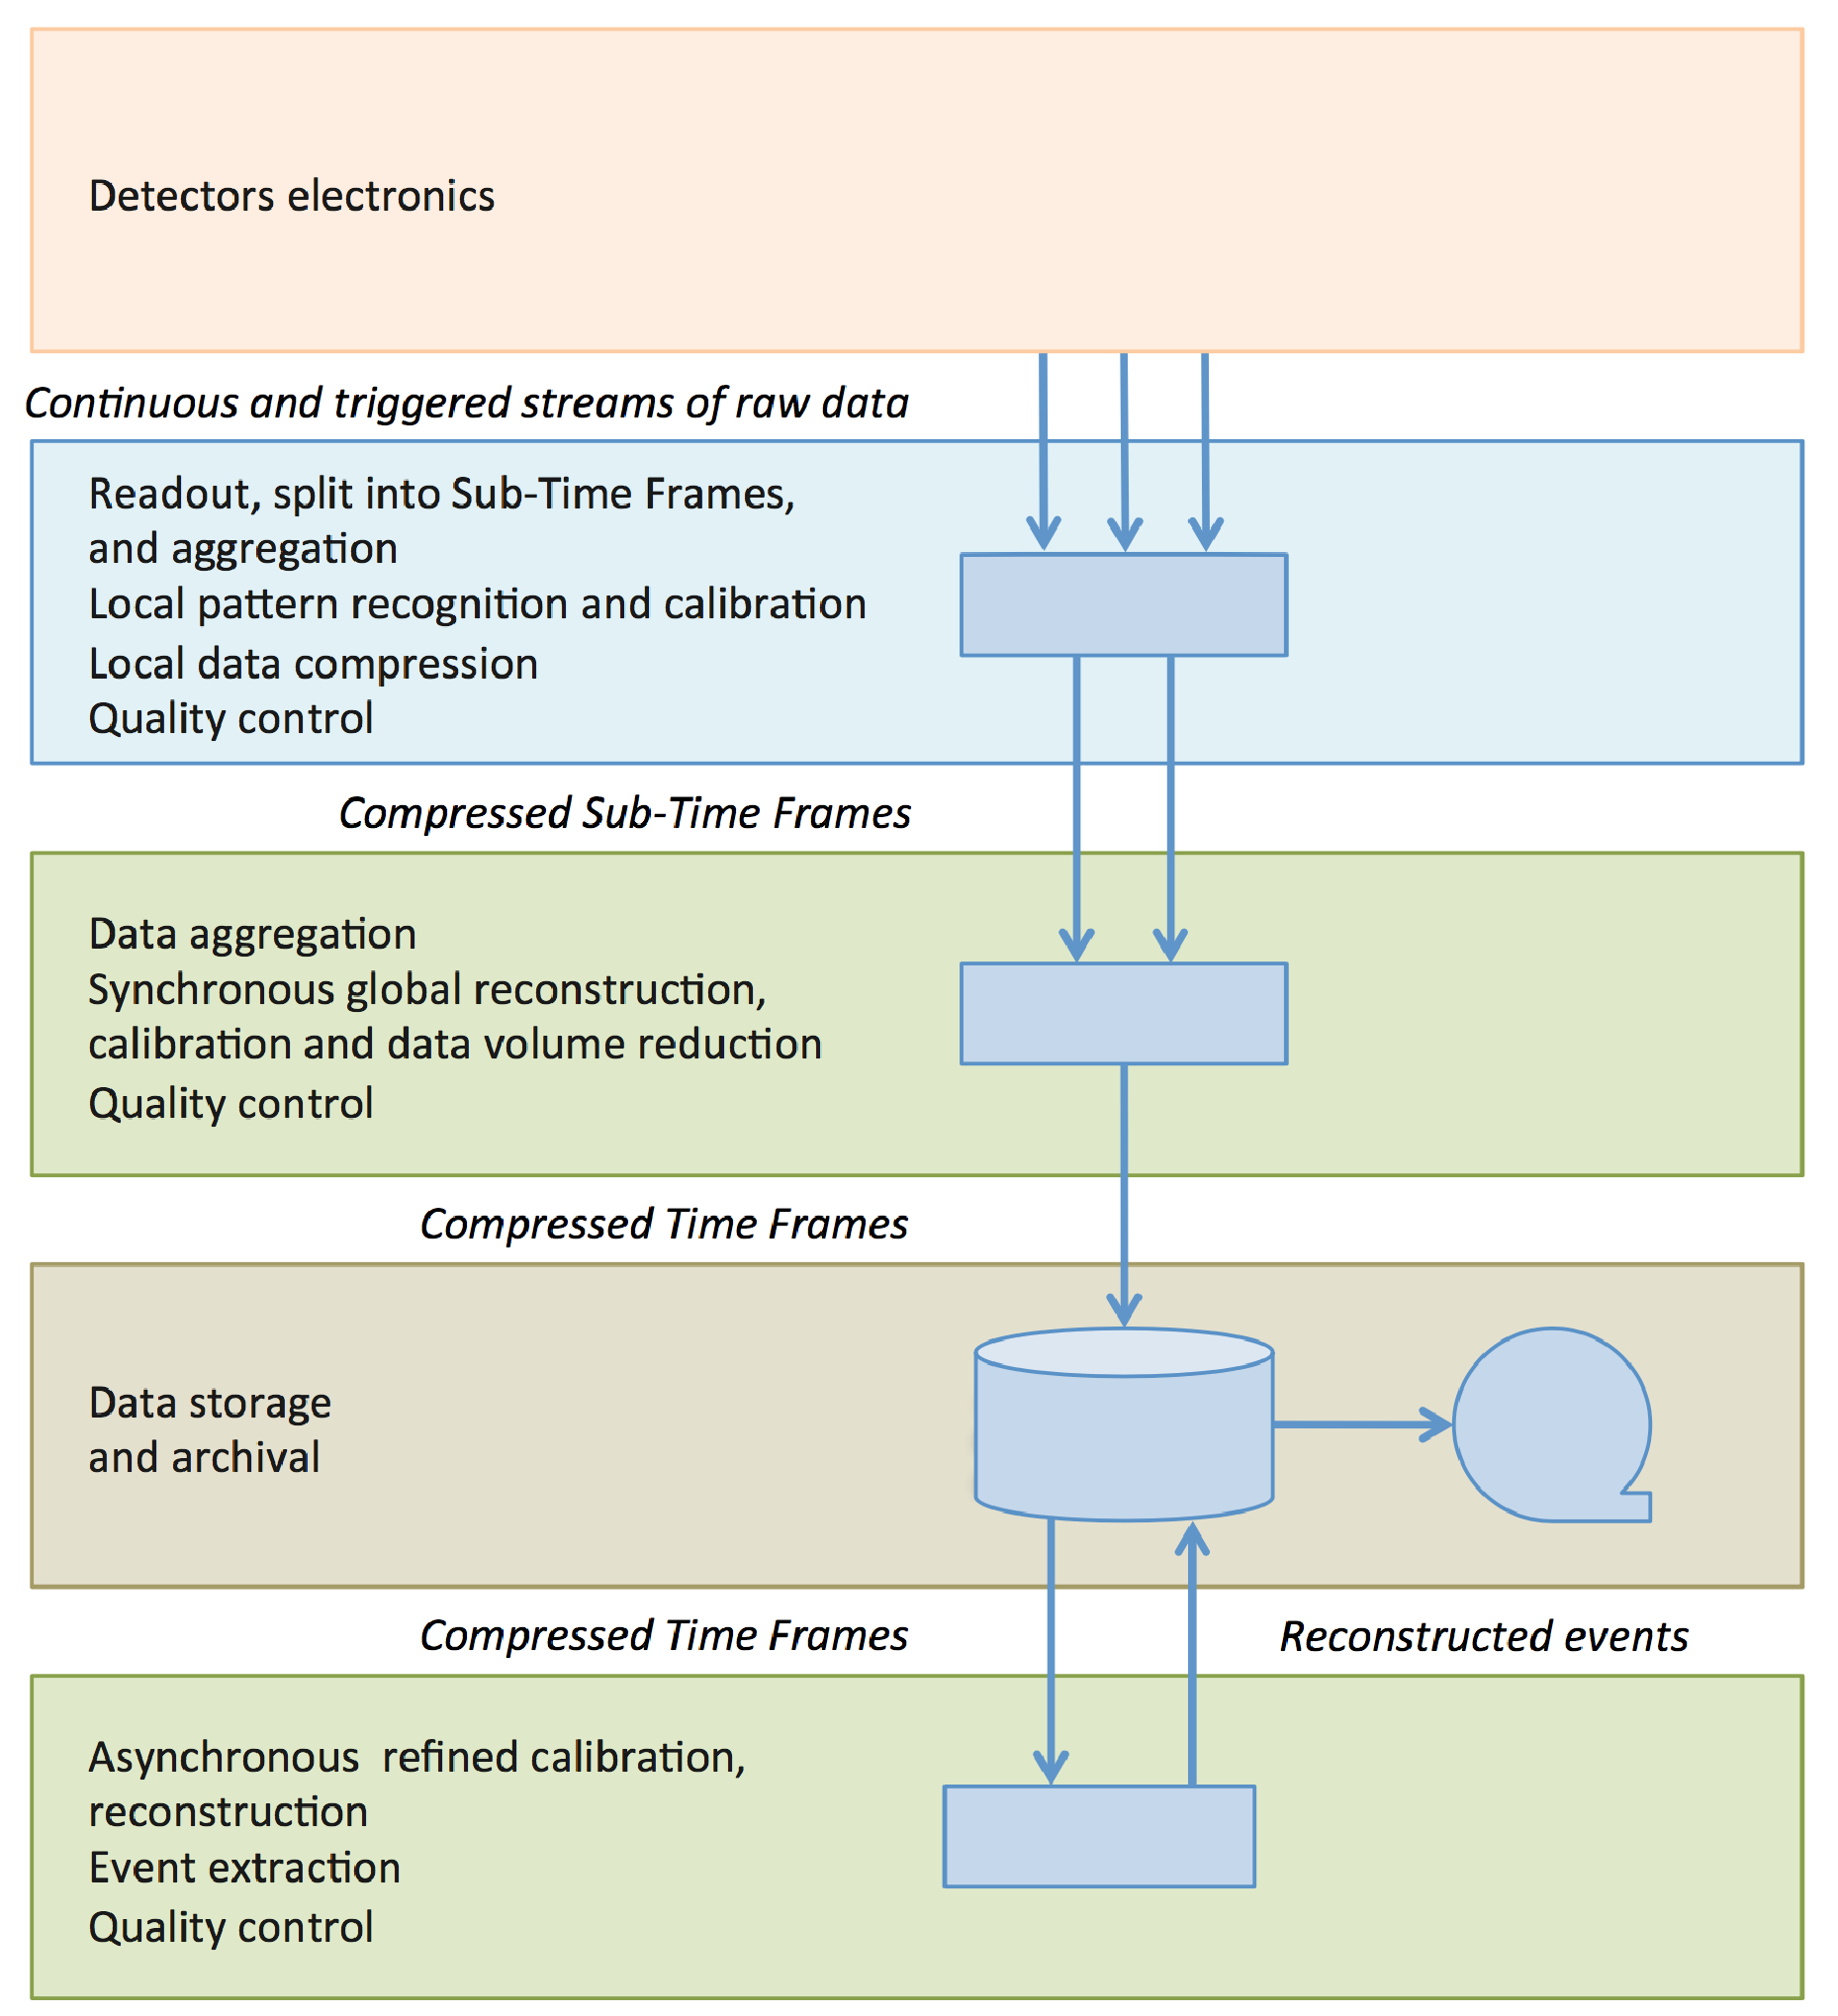
\includegraphics[width=0.95\linewidth]{Chapters/O2/Figs/O2.pdf}
\caption{Sketch of the conceptual structure of the $O^2$ framework. The detectors electronics provides a continuous stream of raw data which is compressed, pre-processed and packed by the read-out logic. Partial information coming from different detectors and systems is aggregated. The full set of data is processed and reconstructed. Up to this step all the computation is performed synchronously. The processed data is then stored and retrieved later for the asynchronous reconstruction.}
\label{fig:O2_sketch}
\end{center}
\end{figure}

Thanks to this fast and partial reconstruction the amount of stored data will be reduced.
% Thanks to this reconstruction procedure, the acquisition trigger will be generated based on finer decisions taken by algorithms able to evaluate the events topology and some physical measurements.
This procedure will replace the hardware trigger, allowing one to perform precise selections focused on getting the maximum signal for rare and otherwise non-triggerable observables.
A finer reconstruction will be performed offline to provide the best resolution possible.
For this finer step the merging of data coming from different detectors will be possible and needed.
% The added complexity and the cross-talk between different systems forces this step to be performed synchronously only during pp collisions.
% An upgraded computing facility installed in place will store the raw data and perform such reconstruction before sending pp data to the CERN storage facility.
Despite an upgraded private computing facility, during Pb-Pb collisions the reconstruction will be performed asynchronously and part of the data processing load will be shared with Tier 0 and Tier 1 computing sites of the WLCG (Worldwide LHC Computing GRID).
Independently from the colliding system type the archival of data will be performed by Tier 0 and Tier 1 facilities.

The combination of synchronous and asynchronous computing and reconstruction steps is well summarized by the name of the software/hardware upgrade project of ALICE.
The Online Offline ($O^2$) project concerns the creation of a common computing system shared by all the ALICE systems and will include a definition of a common computing model, the development of a software framework and the planning and realization of new computing facilities.
The $O^2$ computing facility will be a high-throughput system equipped with heterogeneous computing nodes similar to platforms currently used in several High Performance Computing (HPC) and cloud computing contexts.
The computing nodes will integrate several hardware acceleration technologies, spanning from FPGAs to GPUs.
The $O^2$ software framework will grant an adequate abstraction level so that common code can deliver the same functionality across various platforms.
This characteristic hides part of the complexity deriving from different hardware choices and specializations of machines devoted to particular tasks, in fact the framework layer allows one to make use of multi-core processors (CPUs) in a way almost transparent to the programmer.
Due to fundamental differences between GPU (Graphics Processing Units) and FPGA (Field-Programmable Gate Array) models, the code which is intended to be executed on such accelerators will still require some deep customization.
In order to take full advantage of HPC-like infrastructures, as well as of several laptops or standard desktops connected together, the $O^2$ framework will introduce a concurrent computing model.
While the current WLCG is a distributed computing framework, ideally made of lots of single instruction thread machines, the future development of the ALICE computing framework requires some more tuning to take full advantage of parallel processors.
Since the first era of the HPC the Message Passing Interface has been used as a standard interconnection protocol for computing nodes in computer clusters.
The ALICE computing effort follows a similar approach.
The introduction of such MPI-like process-based framework allows for dynamic spawning of workers, which is baked up with a message passing interface capable of using system buses and network interfaces seamlessly and constitutes the backbone of the new infrastructure.
The $O^2$ project will make ALICE able to tackle the next running conditions without modifying the funding model followed during RUN1 and RUN2.

% \section{Physics objectives of RUN3}
% The $O^2$ project follows the upgrade of the LHC triggered by the increase of statistics necessary for new and improved measurements.
% A requirement of a total integrated luminosity of $13\ nb^{-1}$ in Pb-Pb collisions was formulated with the ALICE Letter Of Intent (LOI) \cite{ALICE_LOI}, split in $10\ nb^{-1}$ at nominal solenoid magnetic field and $3\ nb^{-1}$ at a reduced field of $0.2\ T$.
% These requirements are related to specific performance figures, concerning open heavy flavours, low mass dileptons and quarkonium measurements.
% In particular the plans for $J/\psi$ ($\psi(\mathrm{2S})$) foresee to know its $R_{\mathrm{AA}}$ down to $p_{\mathrm{T}} = 0$ with statistical precision higher than $1\%$ ($10\%$) over the whole rapidity interval and its $\nu_2$ down to $p_{\mathrm{T}} = 0$ with an absolute precision of $0.05$.

\section{Common software efforts}
The $O^2$ project stands on a framework commonly developed by the joint scientific community of several experiments.
$O^2$ aims at reducing the complexity of software deployment and to simplify the exploitation of multi- and many-cores architectures and accelerators, minimizing the development effort to be put.
The $O^2$ software does not rely only on general libraries such as Boost, ROOT and CMake, but also on other two frameworks (Fig. \ref{fig:O2_soft_tree}).
ALFA \cite{alfa} and FairROOT \cite{fairroot} are actively developed by the ALICE and GSI communities.

\begin{figure}[!ht]
\begin{center}
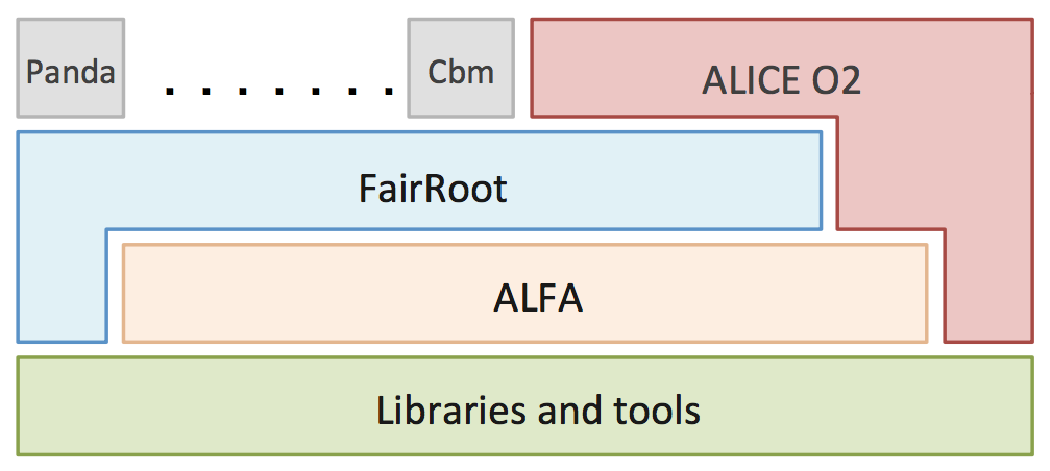
\includegraphics[width=0.8\linewidth]{Chapters/O2/Figs/O2_soft_tree.pdf}
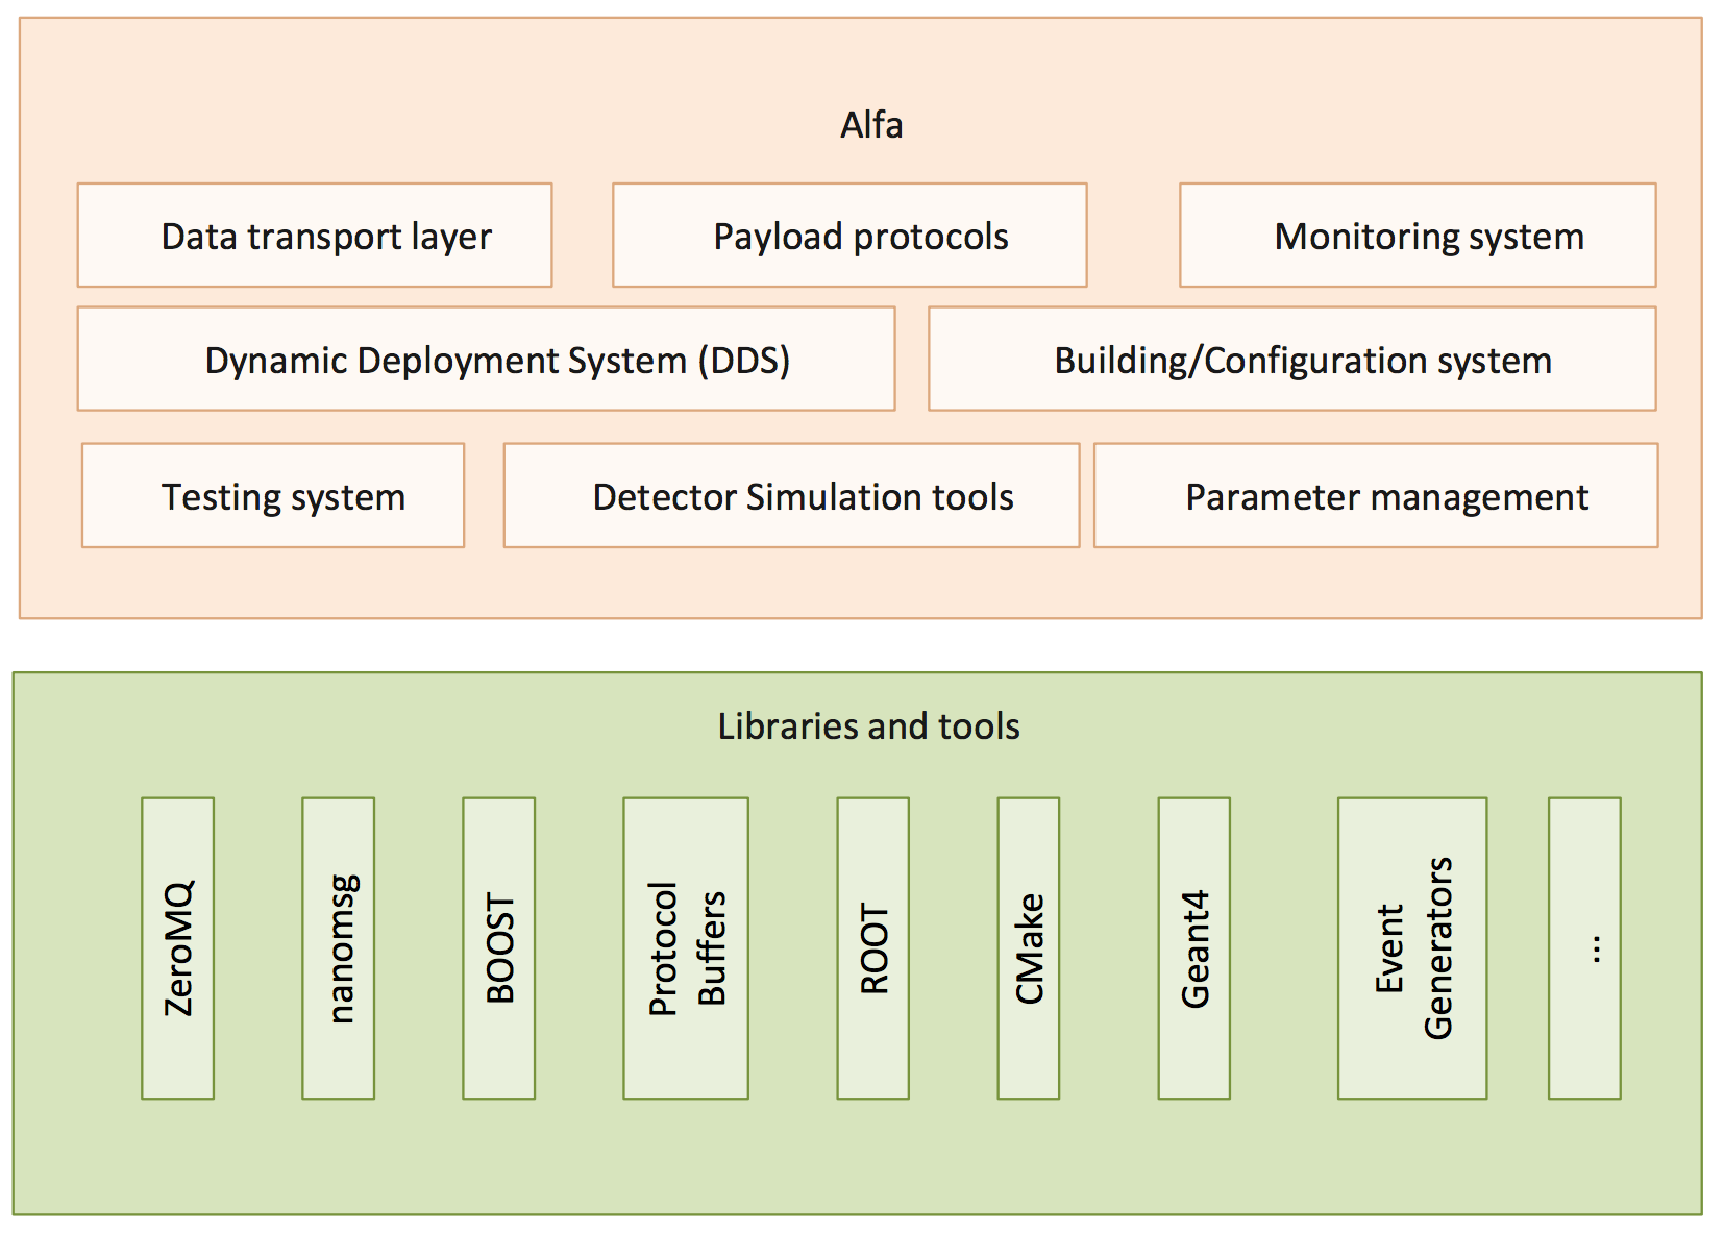
\includegraphics[width=0.7\linewidth]{Chapters/O2/Figs/ALFA.pdf}
\caption{Software topology of the $O^2$ project. $O^2$ stands on several software, sets of libraries and tools. The green boxes represents the low level libraries which constitutes the basis of the software. Some of them are ZeroMQ as message passing protocol, CMake as project build and test manager, Geant4 as particles propagation engine. The orange boxes represents ALFA, developed between ALICE and FAIR. This tool contains a set of high level tools, such as data transportation routines and the dynamic deployment system for the dynamic devices management. The blue box represents FairROOT, an evolution of ROOT focused on improved usability for the end-users. It allows for easy data visualization, storage, offline analysis and more. The ALICE $O^2$ stands on all these elements alongside other collaborations software (Panda, Cbm).}
\label{fig:O2_soft_tree}
\end{center}
\end{figure}

ALFA is a communication and concurrent computing framework.
The handling of an heterogeneous computing system requires two fundamental aspects: communication and coordination.
ALFA provides both aspects and has been developed with high throughput and low latency in mind.
The communication layer is based on the ZeroMQ \cite{zeroMQ} library and allows the passing of binary messages either across network interfaces or between threads within the same machine, by passing memory references.
ZeroMQ is a lightweight message passing interface which is based on a POSIX\footnote{Portable Operating System Interface for uniX. Is a family of standards specified by the IEEE Computer Society for maintaining compatibility between operating systems. POSIX defines the application programming interface (API), along with command line shells and utility interfaces, for software compatibility with variants of Unix and other operating systems.} socket back-end, extending the socket characteristics to make them able to concatenate several messages to optimize transfer rates and to unfold them at destination.
The messages transferred via ZeroMQ have to be serialized as binary buffers.
The available serialization methods are based on Boost, Google's Protocol buffers \cite{googlepb} and ROOT streamers, while the ability to use user defined methods is still left as an option.

The FairROOT framework is an object oriented simulation, reconstruction and data analysis framework  developed for the FAIR experiment at GSI.
It provides core services for Monte Carlo simulations, physics analysis, event visualization and other fundamental tasks.
All the provided functions are accessible in a simple way, in order to simplify the detectors description as well as the creation of analysis workflows.

\section{Data format}
The $O^2$ project introduces a modern approach to the packing of data.
The storage and acquisition model is aimed at getting the highest rate capability possible.
Each storage system packs, with the useful data, a bunch of metadata which constitute a overhead.
Such overhead becomes important for both the transmission and for the storage of data, since part of the bandwidth and/or of the storage capacity is consumed by that.

\begin{figure}[!]
\begin{center}
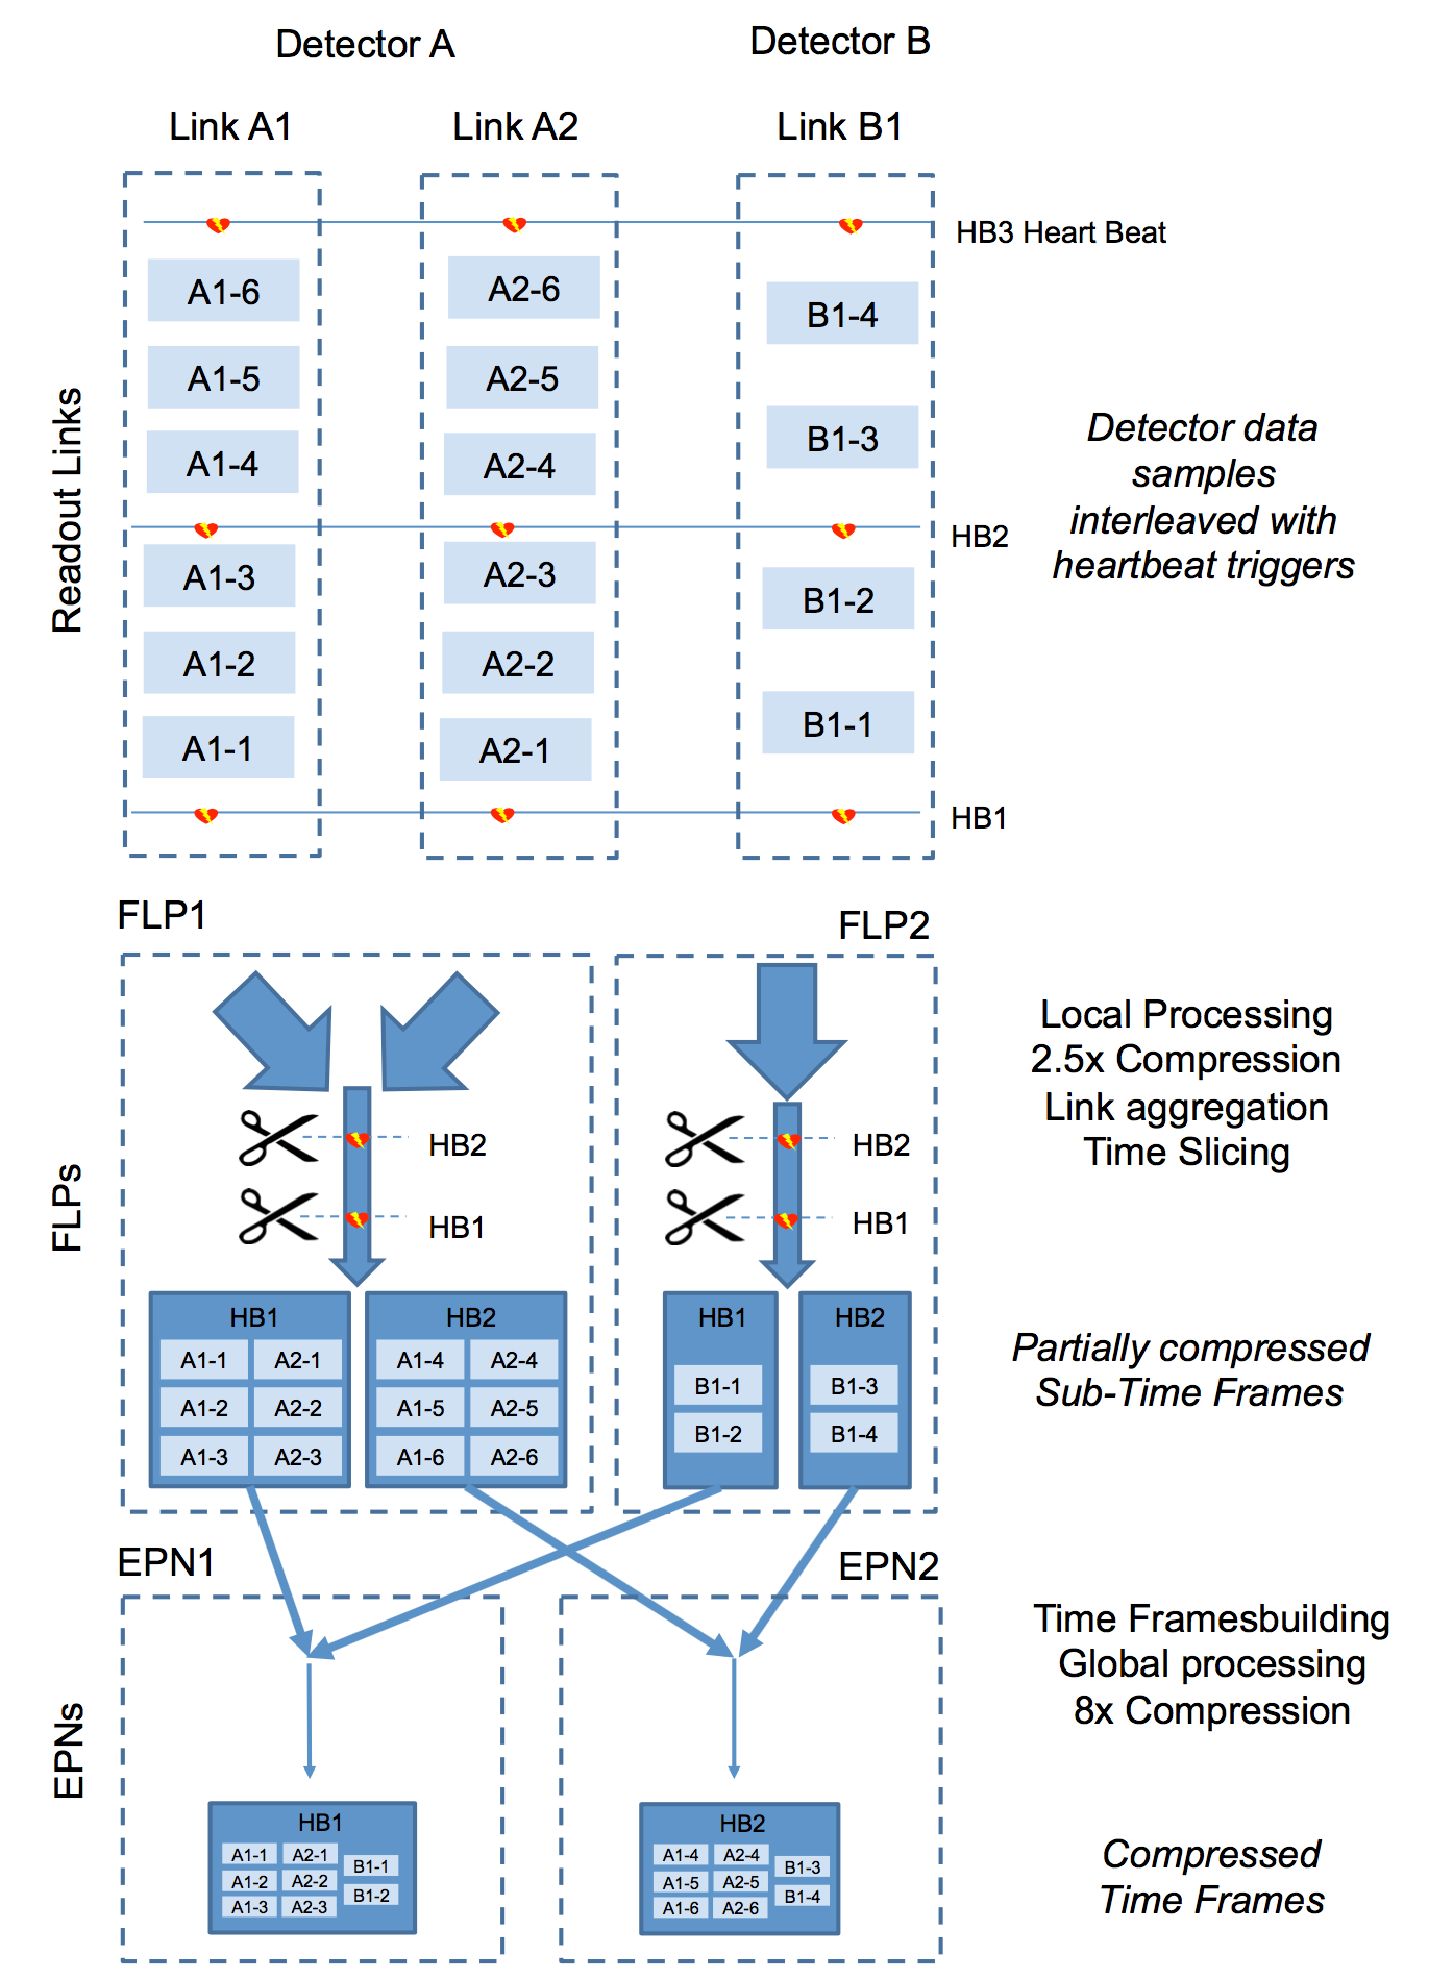
\includegraphics[width=0.9\linewidth]{Chapters/O2/Figs/TF.pdf}
\caption{Sketch representing the acquisition flow with two detectors, A and B. The detector data samples are retrieved by the read-out logic in a continuous fashion, with the addition of heartbeat triggers interleaving for time stamping purposes. At the FLP level each data stream is time sliced, obtaining several patches which are compressed by fast processing and packed in sub TFs. The sub TFs are sent to the EPN farm and then aggregated into global TFs. Each TF has a full set of information regarding a given time interval. A global compression of around $\times14$ is achieved in the process.}
\label{fig:O2_TF}
\end{center}
\end{figure}

The solution introduced by $O^2$ is the so called Time Frame (TF).
The TF is a container defined by two temporal boundaries which define its validity interval (Fig. \ref{fig:O2_TF}).
It packs the data collected by the detectors within the validity interval.
The format chosen for the TF comprehends a header which works as a summary, in order to ease the access to the contained data, and the detector data itself.
The only constraints on the TF content regard the data header specification, while it was chosen to keep as much freedom as possible for what concerns the payload.
For this reason the header must provide a complete description of the whole data structure.
The raw data format cannot be made persistent during acquisition, therefore the raw data flow will be converted in the much more compressed TF format.
% Since both at FLP (First Level Processor) and EPN (Event Processing Node) levels the data format is the TF to allow the interchangeable execution of tasks, $O^2$ foresees the possibility to have sub Time Frames which pack a reduced set of detector data.
% During the LHC RUN3 ALICE will operate in continuous read-out mode.
% The definition of event is difficult, since without performing a full reconstruction it will be difficult to isolate data belonging to each event.
% For this reason the data stream will be split in arbitrary time-frames called SubTimeframes (STF), hence there is a non-null probability for an event data to get split between two STFs.
% Each STF has an header of constant size plus some playload.
% The overhead can be defined as the amount of delivered header data over the size of delivered payload.
% The STF duration has been chosen looking for the best compromise between the overhead fraction and the fraction of lost events.

The data stream of each detector are sent to the First Level Processor (FLP). 
At this level, only the information of one single detector or even part of it is available.
The data format is therefore called Sub-Time Frame (STF).
The processed data are then sent to the Event Processing Node (EPN), which collects the information of all detectors and aggregates them in the TF.
The processing schema is shown in Fig. \ref{fig:O2_Compression}.

% This is mainly needed at the FLP level, when the aggregation of data produced by different detectors is not possible.
% The aggregation, based on the validity intervals of the sub TF, will happen later during the reconstruction stages.
% The TF specification concerns the online part of $O^2$, and defines a standard data format for all the data processed by the reconstruction pipeline up to the stage of writing it in persistent formats.

The TF data format requires all the data to be correctly time flagged, in order to be able to correctly aggregate data within the TF they belong to.
For this reason the detectors raw data flows are interleaved with an heartbeat clock that can be used to attribute a time stamp to the detector data samples.
% At the FLP level the samples belonging to different heartbeat trigger are sliced and packed in STF and sent to the EPNs.
% At the EPN layer the sub TFs coming from different detectors are then aggregated in global TFs.

% All the translation, packing and compression steps described before allow for a strong reduction of the required bandwidth without loosing too much useful data.

\begin{figure}[!ht]
\begin{center}
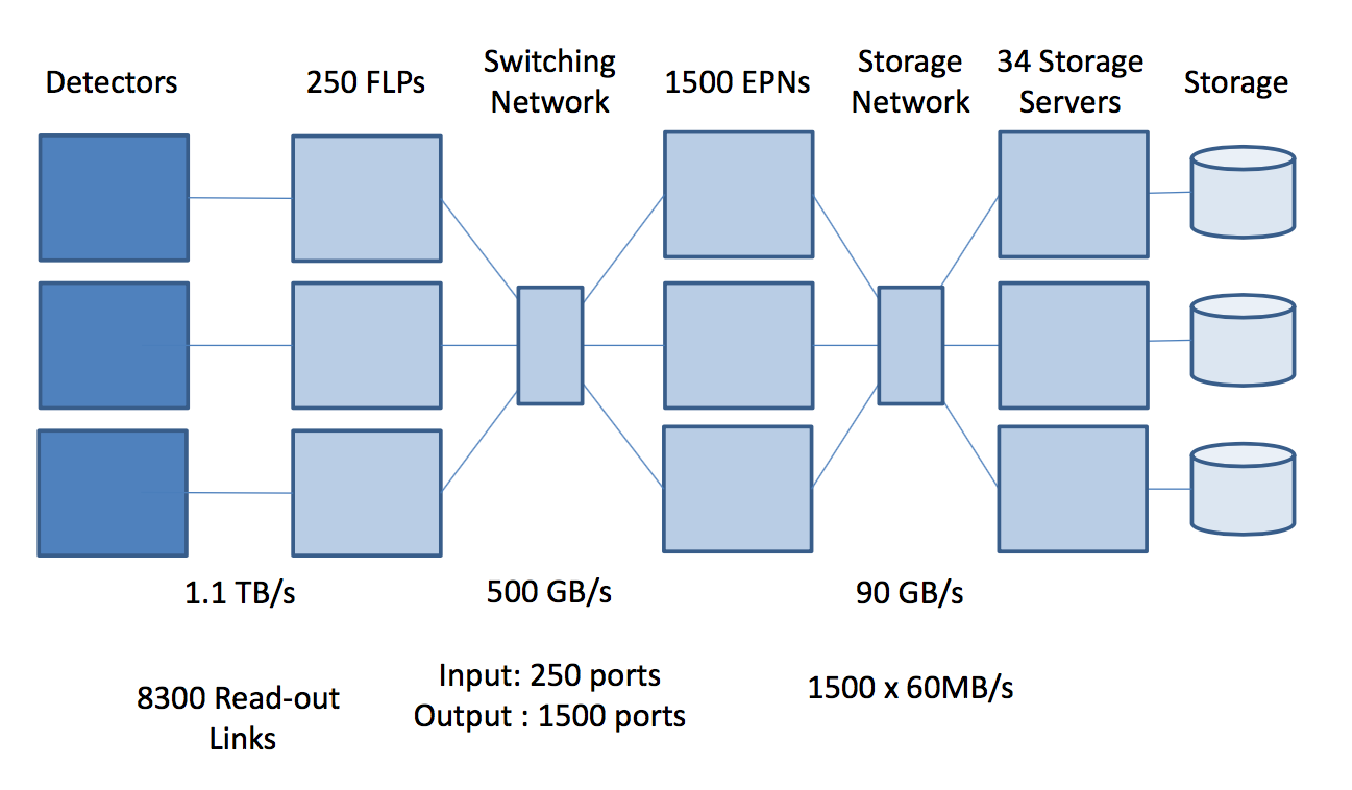
\includegraphics[width=0.75\linewidth]{Chapters/O2/Figs/Compression.pdf}
\caption{Computing infrastructure layers with quoted required input and output bandwidths. An overall factor of compression of $\approx8$ is to be achieved in the process. The network topology is not yet defined by the $O^2$ Technical Design Report since the technology growth is fast enough to require a shorter term planning later during the upgrade.}
\label{fig:O2_Compression}
\end{center}
\end{figure}

A total compression of around $\approx14$ \cite{o2compression} will be possible from the raw data to the storage elements and the first persistent format.

The validity interval of the TF, also called duration, has to be tuned taking into account several criteria:
\begin{itemize}
    \item the TPC drift time causes a loss of $0.1/t_{TF}$, therefore a longer TF is better in this respect;
    \item the calibration data produced during a TF has a fixed size and constitutes a fixed overhead which has to be sent to the Condition Database (CDB). A longer TF would minimize the overhead contribution to data rate and the number of CDB accesses;
    \item the TF should be a multiple of the shortest calibration update period. This value should be the TPC Space Charge Distortion one, scheduled each 5 minutes;
    \item in order to better balance the processing at the EPN level a shorter TF would be better. For the EPNs a buffer of at least three TFs (one receiving, one processing, one sending) is required to avoid dead times.
\end{itemize}
The TF duration will be between $20\ ms$ and $100\ ms$ which corresponds to a rate of $50\ Hz$ to $10\ Hz$.
The number of events packed inside a single TF will reach $1000$ interactions in normal running conditions (Pb-Pb $50\ kHz$).
The resulting TF size will be of $10GB$ on the EPN before compression and the data unusable because of the TPC drift time will be the $0.5\%$ of the total.
Since the EPN farm will be composed by $1500$ machines, each EPN will receive a new TF to process every $30\ s$.

\section{Data Processing Layer}
The tools provided by the default $O^2$ project are intended to be used by experts and require coding skills which are not typical for the physicists community.
Theoretically speaking the tasks are wrappers of part of a bigger algorithm and from now on will be referred as devices.
They are fully described by a bunch of specifications, summarized below:
\begin{enumerate}
    \item The specification of inputs is composed of the indication of the channel of delivery and the kind of data. It is necessary to correctly connect and feed the algorithmic item wrapped in the device. Some devices could be input-less (e.g. MC wrappers, clock generators). A complete set of inputs will be referred as "work item";
    \item The internal state of the device, a set of variables capable of keeping information across several work items. This can be useful for distributed pseudo-random number generators, event counters, histograms and in general any kind of accumulation of results. The initialization of the internal state can be complex without affecting the online performances of the device. In addition some devices, for example those involved in pipeline computations, are "stateless devices", namely devices which do not need to keep a memory of previous computations. Such devices have no internal state;
    \item The computation specification is the algorithm that is called and executed on each complete set of inputs. Any optimization effort has to be put to this part of the device specification, since it represents the main bottleneck being executed in a loop-like fashion. This element is required for any device;
    \item The specification of outputs is similar to the inputs one and consists of the indication of the channel on which the data has to be sent as well as the type of data. The outputs specification is mandatory and the matching between inputs and outputs of different devices has to be perfect to avoid dangling outputs.
\end{enumerate}

In this approach each device has to implement one and only one basic function.
The devices are intended to be self contained and atomic.
This opens up the possibility to spawn device clones or to kill unused devices to free resources for other tasks.
For example if a given device (or a group of homologous devices) starts starving ($e.g.$ the CPU set waits for data since the computation is too fast with respect to the data flow) and a loss of computing efficiency is measured, it might be killed by a manager process.
Similarly if a group of devices cannot cope with the input rate, the manager process can add some more in order to improve the throughput of the whole set of devices using the resources freed up by the killing of starving devices.

Within the FairROOT framework, several utilities and libraries have already been implemented to simplify the configuration of new devices.
In $O^2$ the description of the devices is even more trasparent to the end user thanks to an additional framework called Data Processing Layer (DPL).
The DPL hides much of the complexity required by the MPI-like FairROOT devices.
After some development efforts, the residual complexity left to the programmer by the DPL is negligible.
Using advanced C++ techniques, available in the 11, 14 and 17 standards, the description of input and output channels is similar to the initialization of a list, while implementing the initialization and data processing functions is as complex as the required algorithm itself.
The typical complexity of concurrent computing software framework is almost completely hidden, leaving much of the coding focus to the algorithmic part.
During my thesis, I also participated in the effort of writing high level routines that can be easily adopted by the DPL framework to simplify the serialization of the messages. 
Such routines, based on \code{boost}, were extensively tested and are currently used many detector and subsystem-specific code and are requested to be included in the FairROOT core by its developers team.

The DPL approach is being adopted by most part of the detectors and the systems included in the $O^2$ upgrade project, and the upgraded muon trigger software follows this schema.

\section{Muon tagging algorithm}
\label{MTR_tagging}
The pre-upgrade offline muon tagging algorithm was intended to be executed during reconstruction, in an asynchronous computing model.
Within the $O^2$ upgrade this algorithm will be modified to be fed with information computed synchronously strongly improving the muon tagging capabilities of the system.
It is based on the matching between tracks reconstructed in the muon tracker and the tracklets (straight tracks) reconstructed in the MTR.
The tracks reconstructed within the muon chambers are obtained using a Kalman Filter algorithm.
Since the five stations of muon chambers are placed upstream, inside and downstream of the dipole magnet, the reconstructed tracks are curved.
The reconstructed tracks are extrapolated towards the muon trigger system.
These informations are then matched with the tracklets generated using the MTR data.
% A tracklet is a set of crossing point and 3D slope, describing a straight segment.
% The muon chamber tracks extrapolation uses the same format.
The muon identification criteria is based on the fact that only the muon chamber tracks which are found to correspond to a muon trigger one are to be considered muons, since it is unlikely for other particles to cross the $1.2m$ thick iron wall between the two stations of the muon trigger (Fig. \ref{fig:MTR_old}).

\begin{figure}[!ht]
\begin{center}
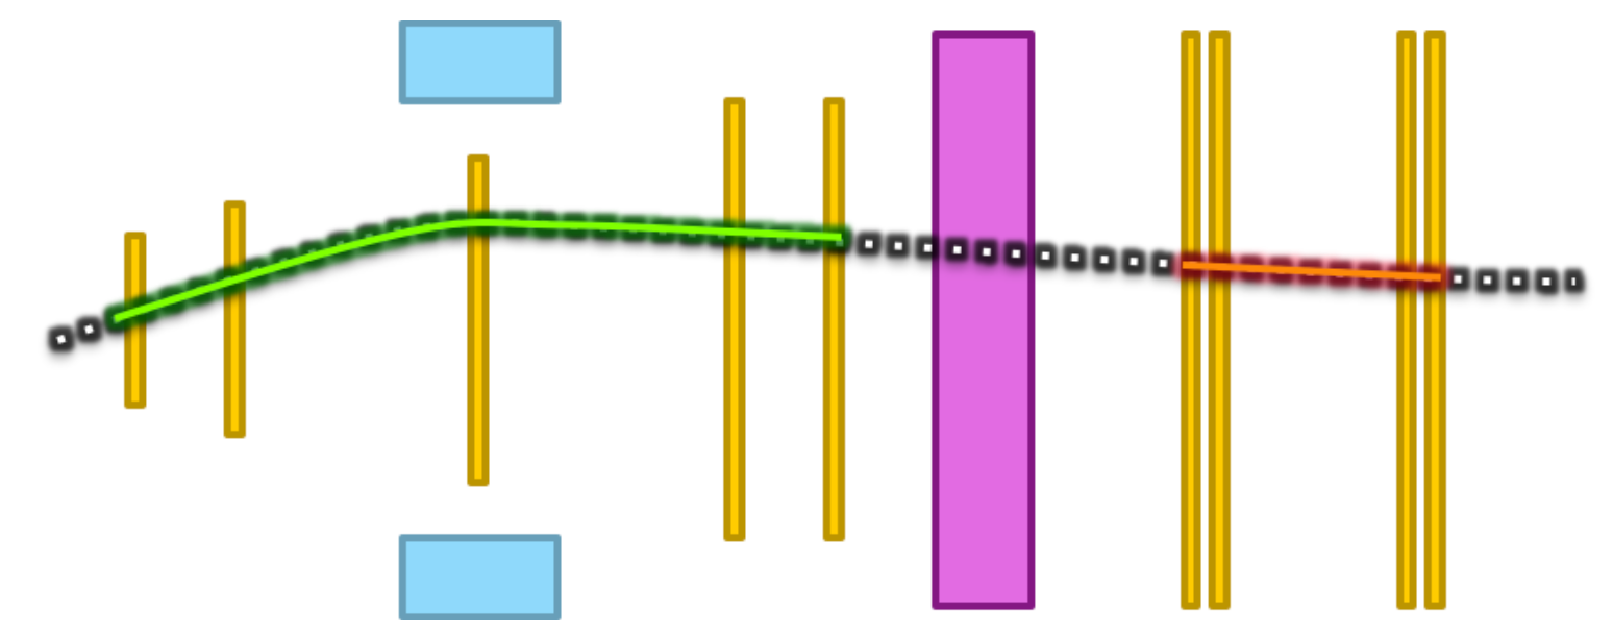
\includegraphics[width=0.9\linewidth]{Chapters/O2/Figs/MTR_logic.pdf}
\caption{In this picture the muon chamber and muon trigger planes are represented in yellow, the iron wall in purple and the dipole is shown in blue. The dashed line represents the true trajectory of the muon. The green line is the reconstructed track within the muon chambers, while the orange line is the tracklet reconstructed in the muon trigger.}
\label{fig:MTR_old}
\end{center}
\end{figure}

The generation of the tracklets in MTR was based on the MTR trigger algorithm, which is in turn based on the Local Boards, which collect the information of the fired strip in a projective region in the four detection plane. 
When a particle fires a strip in the first chamber, the local board searches for aligned strips in the other chambers, combining the information of the adjacent  local boards in the bending plane. From this information the algorithm computes a hit position in the first chamber and a deviation, i.e. a tracklet.
This algorithm, however, provides at most 1 response (and therefore one tracklet) per local board. In the case where more than one tracks crosses the same local board, the algorithm is tuned to chose the combination of hits providing the minimum deviation (i.e. largest $p_\mathrm{T}$) in order to keep the highest trigger efficiency. 
This however might result in a reconstruction of just one track, as shown in figure \ref{fig:MTR_loss}, or of a fake track that does not match any of the two real tracks.
This limitation affects the most central heavy-ion collisions, where the large particle multiplicity results in a larger probability of having to muons crossing the same LB.
The inefficiency was then caused by an algorithmic feature more than by the detector itself.

\begin{figure}[!ht]
\begin{center}
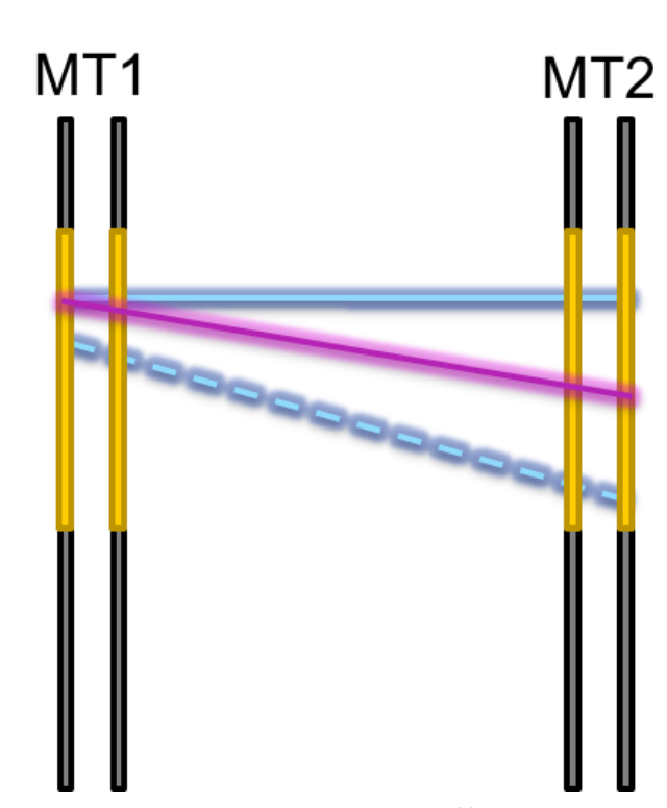
\includegraphics[width=0.5\linewidth]{Chapters/O2/Figs/MTR_old.pdf}
\caption{The MTR planes are shown in grey, while the hit local board is highlighted in yellow. Two real trajectories are represented by the lines. The algorithm is tuned to select the less sloped track in case of ambiguity, hence only the solid blue track would be recorded.}
\label{fig:MTR_loss}
\end{center}
\end{figure}

Some development of an algorithm capable of recovering the performance loss in the most central events was performed but never put in the production code.
% Given the much higher luminosity and interaction rate foreseen for the LHC RUN3, this aspect should be fixed by the new implementation of the MID algorithm.
The complex solution of implementing a tracking algorithm in using the former MTR, excluded for RUN2, was indeed the proposed solution for RUN3 running conditions.
% The approach used during RUN2 allows for easier measurement of the matching efficiency, since the tracklets which get evaluated to generate the trigger signal are the same that offline are matched with the muon tracker tracks.
% Implementing a tracking algorithm brings in the possibility to generate fake tracks which might match with muon tracker tracks.
% This aspect causes some additional hassle in the evaluation of the matching efficiency and that solution was discarded for RUN2 operations.
% With RUN3 such solution has become necessary and was implemented.

\section{From Muon TRigger to Muon IDentifier}
In the Run3, the MTR will lose its functionality of a triggering detector\footnote{although the possibility of providing a very basic trigger was kept in the electronics, mainly for studying muon production in ultra-peripheral Pb-Pb collisions}, and it will only be used to provide muon identification. 
Its name will be changed accordingly to reflect the change of functionality, thus passing from Muon TRigger to Muon IDentifier (MID).
% The name of the ALICE muon trigger (MTR) will be modified from the introduction of the $O^2$ project.
% This change of nomenclature is related to a change of its online functions.
% The muon trigger provided various online acquisition triggers based on the detection of muons and worked as a muon tagger for the muon chambers tracks.
% The MTR will see the upgrade of read-out electronics, already presented in previous chapters.
% In addition to this hardware upgrade, the online function of the MTR system will change.
% The MTR system will no longer provide an online trigger system for ALICE, since the acquisition paradigm will move to trigger-less.
% Instead the system will become a stand alone muon tracking system.
% Even if the tracking resolution of the muon trigger system is lower than that of the muon tracker and that of the future MFT (Muon Forward Tracker), the muon identification task will be achieved by the MTR which will then become the MID (Muon IDentifier).
The muon identification (and hadron rejection) task will be performed combining data coming from the MCH and MID detectors.
The addition of the Muon Forward Tracker (MFT) \cite{CERN-LHCC-2015-001} will improve the tracks resolution closer to the interaction point and make it possible to resolve secondary vertexes.
The tracks reconstructed with MCH data will be identified as muons if a compatible track in the MID detector is present.
This task will be performed online, processing and reconstructing around $300\ MB/s$ \cite{Buncic:2011297} of data in Pb-Pb collisions.
The acquisition/reconstruction workflow is represented in figure \ref{fig:O2_sketch}.
Data recorded by the FEE will be acquired via several GBTx link by the Common Readout Units (CRU), each one processing one half of the MID (inside and outside).
The CRUs are implemented as PCI express boards equipped with two external GBTx ports and an on-board Altera Arria X FPGA.
The CRUs will be installed in two dual CPU machines called First Level Processors (the FLPs) which will be placed in the counting rooms placed over the ALICE cavern, as close as possible to the detectors.
The CRUs will perform the coding of the input stream in a binary format which can be sent and processed by the FLP (Fig. \ref{fig:O2_CRU}).
Zero suppression and noisy/dead channels detection/suppression will be performed by the CRU.
Finally, at the EPN level, the combination of MID data with data coming from other detectors will be possible.

\begin{figure}[!ht]
\begin{center}
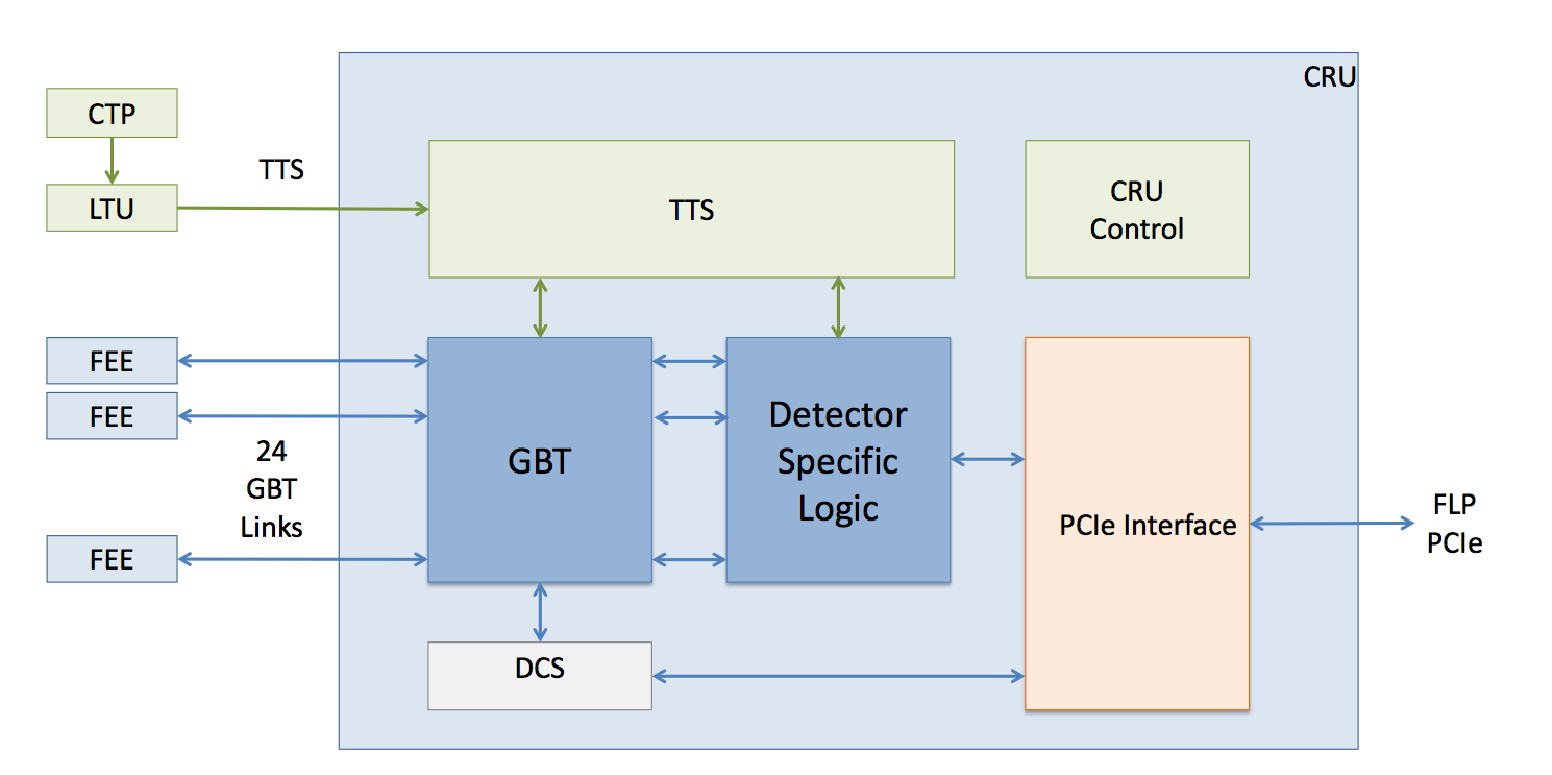
\includegraphics[width=0.9\linewidth]{Chapters/O2/Figs/CRU.pdf}
\caption{Detailed sketch of a generic Common Readout Unit (CRU). The Front End Electronics (FEE) are connected to the CRU through 24 embedded GBT links. The green boxes are connected to the Central trigger Processor (CTP) and deliver timing information to time tag the raw data flow, performed by the detector specific logic. The raw data is translated in a binary format which can be processed by the FLP CPUs. The ouput of the CRU is performed by a standard PCI Express link.}
\label{fig:O2_CRU}
\end{center}
\end{figure}

\section{MID raw data format}
The MID data format follows such data format follows the directives of $O^2$ for what concerns the description of the payload by means of headers.
A top level header defines the binary intervals at which what kind of information is found and constitutes a constant size overhead.
The management of data inside the binary payload follows a tree pattern.
At each branching of the pattern a description (header) describes the positions of the following branches.
In turn each branch provides a self description needed to deserialize and decode the content.
The data format requires a sequential access in order to correctly map its content to meaningful variables and structures.
The data format has an implicit zero suppression, since only the hit strips are coded in a bit pattern which is then sent.

\begin{figure}[!ht]
\begin{center}
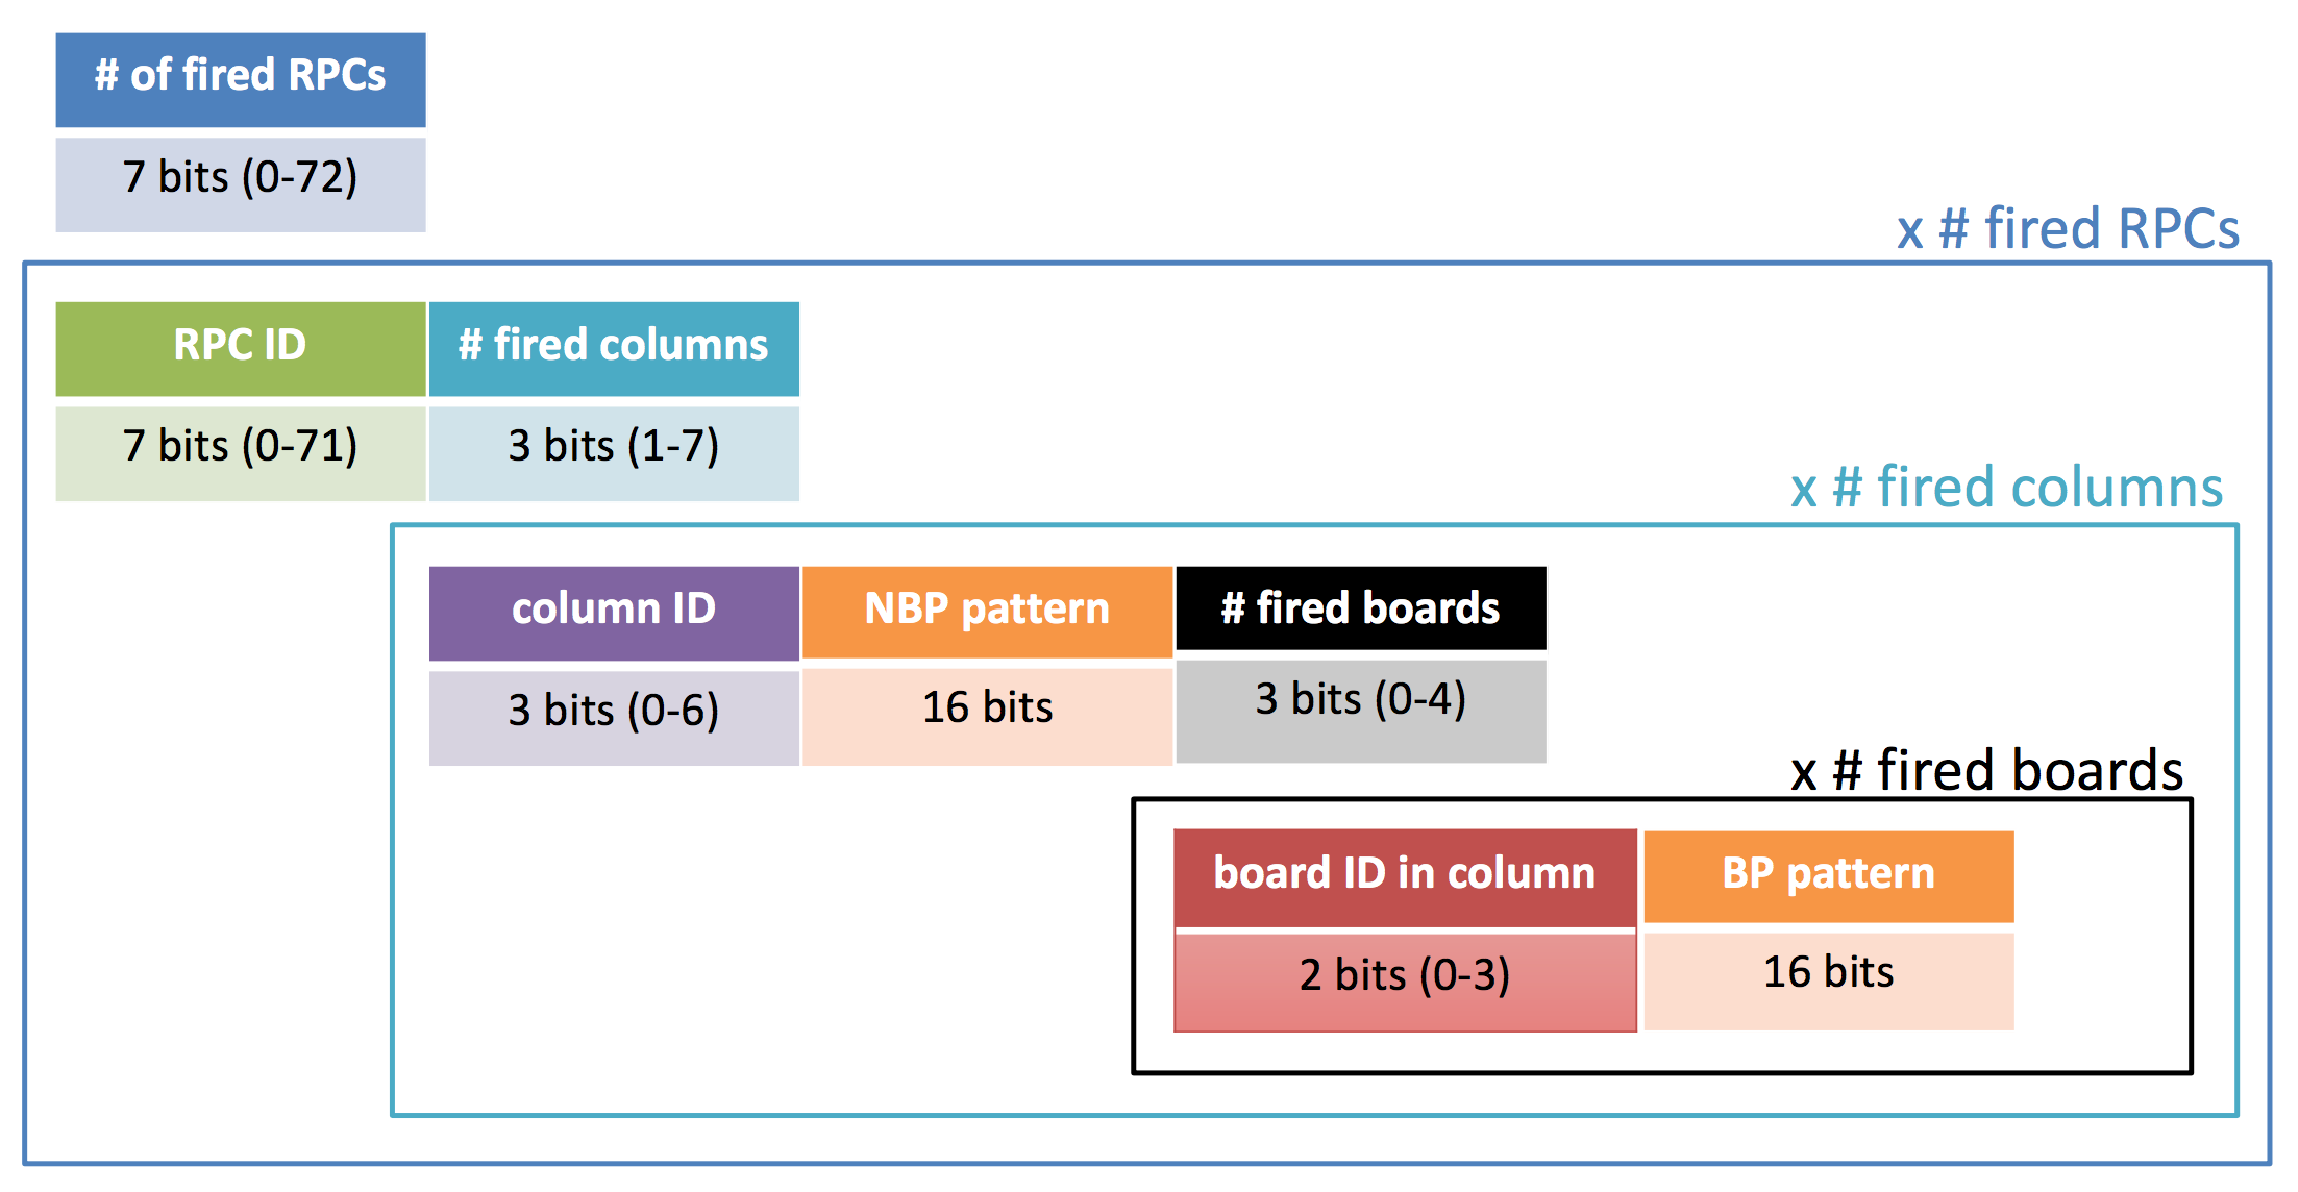
\includegraphics[width=0.99\linewidth]{Chapters/O2/Figs/MID_format_2.pdf}
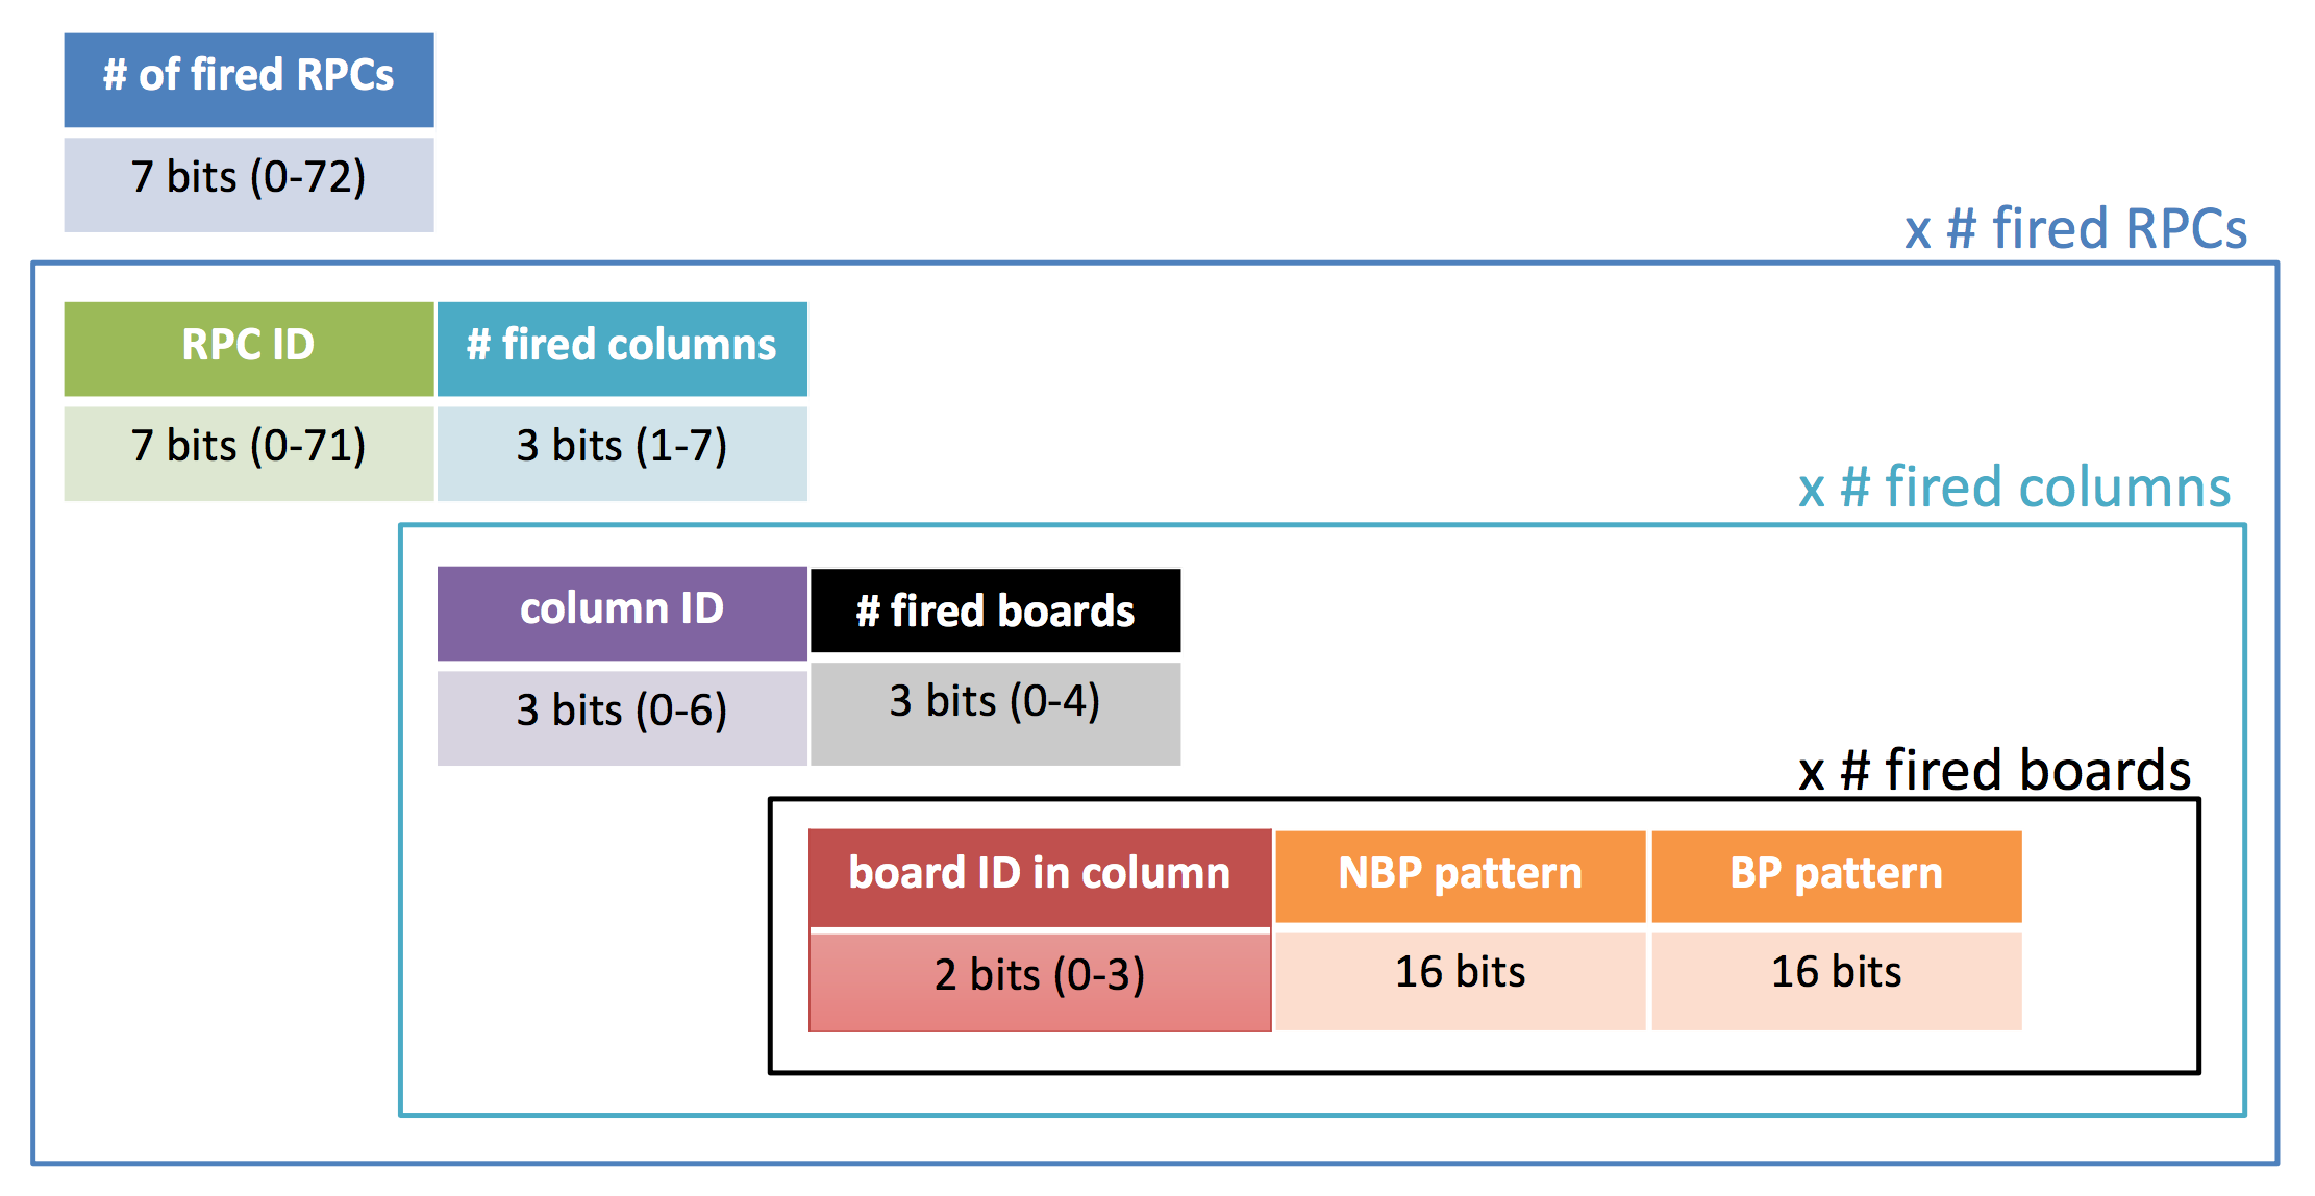
\includegraphics[width=0.99\linewidth]{Chapters/O2/Figs/MID_format_1.pdf}
\caption{Two CRU data format proposals. 
In the first option only one non bending pattern is sent from the CRU to the FLP, while the FEE sends to the CRU several copies of the same pattern since the horizontal strips are read by several local boards each. The CRU has to perform some operation in order to combine the multiple non bending plane patterns into a single one.
The second format foresees to send to the FLP several non bending plane patterns, which are combined by the FLP itself.}
\label{fig:MID_CRU_DF}
\end{center}
\end{figure}

Each side of the MID serializes the information using as top level header the number of fired RPCs, which corresponds to the number of following branches.
Each branch representing an RPC provides an header which quotes the RPC ID and the number of columns fired within that RPC (see Fig. \ref{fig:MID_CRU_DF}).
Another branch level represents each of the fired columns and for each column both the column ID and the number of fired Local Boards (LB).
The deepest branch level represents the LBs by giving the LB ID and the bit patterns of the LB.
The patterns correspond to strip in the bending and non-bending direction. 
It is worth noting that the non-bending strip can cross several local boards, so each pattern is a copy, in that local board, of the non-bending information.
In an alternative proposal, the non-bending information is stored only once per column (see Fig. \ref{fig:MID_CRU_DF} bottom). 
The advantage is that the information is not replicated, but in this case any mismatch in the local copy of the NB strip needs to be monitored at the CRU level.
It is also worth noting that all of the patterns are coded in 16 bits, although some LBs are equipped with only 8 strips in the NB direction.
% The patterns correspond to bending and non-bending strip directions and each pattern is coded in 16 bits, which are not always completely filled.
% In fact some LBs are equipped in a given direction with less than 16 strips.
In that case the pattern gets filled accordingly to the hits and the exceeding bits are set to 0.

As already stated, the MID RPCs require to perform two kinds of calibration events in order to detect problematic channels.
The issues can be either channels which starts to count continuously because of a discharge in the chamber or channels which stops counting because of detector or electronics failures.
The characteristics of the two kinds of calibration events are intended to address the detection of both issues.
% The first kind of calibration run is performed when no collision is happening (e.g. between two interactions).
% In such situation the noisy channels can be detected since they would be the only ones counting.
In one case the read-out of the detector is triggered asynchronously with respect to an interaction.
In the absence of a cosmic event, only noisy channel will respond in this case.
In a second case, the FEE injects charge above the threshold in all channels to check whether they are responsive or not.
% The second kind of calibration run is performed using a FEE feature which provides an independent circuitry to inject an electric charge in the strip itself.
During this calibration event all the strips are stimulated, therefore expected to be counting.
This allows one to detect the presence of dead channels.
The chosen MID raw data format is not efficient for the second kind of calibration event.
In fact, since the dead channels are expected to be a small part of the total, during such events the bit patterns of almost the whole detector should be transferred.
In order to optimize the data delivery process, by reducing the amount of useless information being sent, an additional bit can be delivered in order to flag the message payload as "straight" or "inverted".
In the first case nothing changes and the overhead of the data format would be increased of 1 bit.
In the second case only the dead channels are sent as if they would have been the only channels switched on.
Thanks to the additional bit, the decoder will be able to invert the message to obtain the correct information.
% In addition, in case of bandwidth  bottlenecks, the inversion bit could become useful in case of high MID occupancy.
% In case more than $50\%$ of the detector is switched on, the FEE could decide to deliver the inverted bit pattern flagged accordingly.
% The expected MID occupancy is however expected to be low enough to discard the usage of the inversion bit for any event but for the calibration runs of second type.

\section{MID reconstruction pipeline}
The MID reconstruction pipeline is an algorithm which, from a global point of view, should convert the digits streams obtained from the CRUs to a stream of 3D tracks representing the detected muons.
The digits stream coming from the CRU is decoded and, in case of the special software trigger, the noisy and dead channels are computed.
The detection of noisy channels will allow for the generation of a mask that will have to be transferred to the local boards. 
This is fundamental because the presence of noise increases the bandwidth from the detector readout to the CRU, eventually leading to a saturation. 
The details of the transfer, however, are still under investigation. 
The information on dead channels and masks needs to be permanently stored so that it will become available for simulation and efficiency evaluation purposes. 
This will most likely be done in the Condition DataBase (CDB).
Moreover, the detection of dead and noisy channels will be the first step of the Quality Control (QC) of the detector, since it allows one to pinpoint hot spots and dead zones of the RPC chambers.
% This procedure is needed for two reasons. 
% First of all one wants to keep track of problematic strips in the CDB (Condition DataBase) to be able to highlight problematic RPC chambers and to detect hot spots and/or dead zones which can both lead to a loss of efficiency. 
% Moreover, concerning the noisy channels, their reading are not significant from a tracking point of view since they simulate a particle crossing which did not happen, hence one wants to mask out noisy channels in order to help the tracking algorithm. 
% While the record of the noisy and dead channels can be performed in a relaxed way, the masking of noisy channels should be capable of sustaining the same rate of the inputs in order to avoid the introduction of delays. 
% The applied mask has to be stored in the CDB as well, alongside a temporal validity range, to allow a granular reconstruction of the MID running condition for simulation adn efficiency evaluation purposes.
The reconstruction steps for the MID are intended to be mainly (if not globally) executed on the detector FLPs.
The MID will be equipped with one FLP per side (inside and outside) which won't be equipped with a cross connection, hence won't be able to exchange data.
For this reason the MID has to be considered as a pair of independent detectors.
Only at the EPN level data coming from both sides will be merged and combined.

\begin{figure}[!ht]
\begin{center}
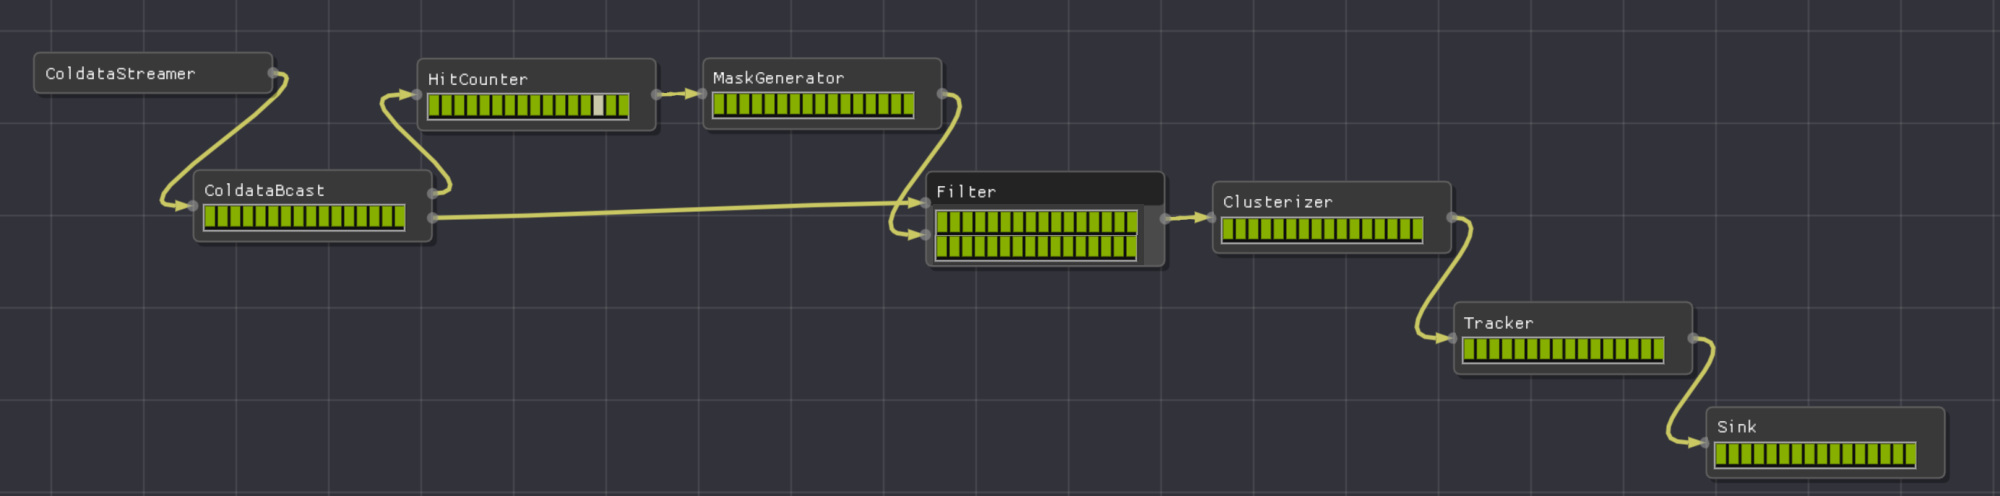
\includegraphics[width=1\linewidth]{Chapters/O2/Figs/MID_workflow.pdf}
\caption{Schema of the MID reconstruction workflow obtained from the DPL Graphic User Interface (GUI). This workflow is intended to be executed in the FLP. Each box represents a device and the arrows represent a data stream. The first device, called ColDataStreamer, is a random generator of fake CRU messages able to emulate the CRU behaviour for testing purposes. The upper branch represents the asynchronous mask computing stage of the workflow. The last device, called sink, represents the connection to the EPN nodes and the second online processing step.}
\label{fig:MID_workflow}
\end{center}
\end{figure}

Regarding the acquisition, some logic steps to perform the conversion have been defined, in order to provide atomic computation items able to be packed in deployable and modular devices:
\begin{itemize}
    \item The digits coming from the CRU are cloned towards two branches.
    The first branch leads to the mask generation and can be asynchronous with respect to the input data flow.
    The second branch has to present limited latency to avoid starvation of the following reconstruction devices;
    \item The mask generation branch begins with a rate computer, namely a device with an internal state which works as a per-strip counter.
    % The counters are sent to a mask generator device which reads the counters and spots the noisy channels;
	Two counter sets are available, one for the noisy and the other for the dead channels, incremented during the corresponding special events;
    \item  A mask generator devices reads the recorded counters and spots dead and noisy channels by looking at the scalers incremented during calibration runs.
    % Two scalers sets will be available, the first being filled by the readings of the dead channels test, the second by the noisy channels one.
    % The channels switched on when no collision is happening are marked as noisy and propagated to the mask.
    % The channels not counting during the injection of charge in the electronics are marked as dead.
    The mask is sent to a filter device;
    \item A filter device is capable of applying the mask to the incoming digits.
    The application of the mask is the logic AND between the incoming patterns and the corresponding mask.
    In case no mask is present, or the mask is empty, the digits should simply be passed through as fast as possible.
    Achieving the lowest latency on this device is crucial;
    \item The stream of masked digits is then processed by a clusterizer device. The binary digits are here converted to 2D clusters, computing the centroids of the hits clusters. 
    % The third coordinate of the cluster is extrapolated from the detector geometry and added to the planar coordinates.
    This computing step is a typical high throughput stateless computation;
    \item The 2D clusters in the local RPC reference frame are passed to a device that converts it in 3D clusters in the global reference frame and preforms the tracking through a Kalman Filter algorithm.
    The generated tracks are sent to the following reconstruction steps executed by the EPNs.
\end{itemize}

The MID reconstruction pipeline has been developed within the DPL framework.
A schema of this pipeline, as provided by the DPL Graphical User Interface (GUI) itself, is shown in \ref{fig:MID_workflow}.

\section{MID reconstruction performances}
% The MID algorithm has to be validate in order to provide a performance similar to the old MTR offline reconstruction, with the added rate capability.
The MID reconstruction algorithm is new compared with what was used for MTR, which was entirely based on the trigger algorithm.
Both the clustering and the tracking algorithms need to be validated in Monte Carlo (MC) simulations. 
The framework for MC simulation for MID is work in progress, but, since the detector geometry and segmentation did not change with respect to MTR, the Run2 simulation can be used for the validation of the algorithms. 
In particular, a custom MC production using a \jpsi parametrization as input is used. 
The crossing points of the tracks in the RPCs are used by the MID digitizer algorithm to generate the digits on which the MID reconstruction chain is applied. 
The reconstructed clusters and tracks are then compared to the MC impact point and track parameters to estimate the residuals. 
The final aim is to study:
\begin{itemize}
    \item The resolution of the algorithm in four variables: 
    \begin{itemize}
        \item the cluster resolution\footnote{The resolution is defined as the difference between the real parameters of the track and the reconstructed ones.} (along x and y);
        \item the track resolution, i.e. the resolution on the track position (mainly along x and y) and slopes along the bending and non bending plane;
    \end{itemize}
    % $x$ and $y$ first crossing resolution and vertical and horizontal slope. The resolution should be studied both as a function of the detector element and of cinematic variables of the reconstructed particle. 
    
    \item The muon reconstruction efficiency;
    \item The fraction of fake tracks, i.e. tracks reconstructed with the wrong parameters by mixing real hits from different particles or noise. The study should be performed as a function of the particle multiplicity in the MID chambers.
\end{itemize}

Some of these tests have already been performed and will be presented.
The methodology for the tests that are not accomplished yet will be discussed as well.

\subsection{Cluster residuals}
% The overall reconstruction resolution is related to the cluster size.
% Usually the cluster size is defined by the number of adjacent strips which are fired by a given particle.
% Since such definition is not able to take into account different strip pitches, like the ones installed in the MID, a different definition is given and adopted from now on.
% The cluster size is defined as the maximum distance between the first and the last strips of the cluster, both in $x$ and $y$ directions.

The MID electronics does not provide any information on the deposited charge. 
For this reason, a charge centroid cannot be computed and the cluster centroid is purely geometrical.
The centroids coordinates are computed as the average of the coordinates of the strips.
Since a flat distribution of crossing probability has to be assumed within the cluster extension, the resolution is directly proportional to the cluster extension via the relation $\frac{CS}{\sqrt{12}}$ where $CS$ is the cluster size.
% The cluster size has been studied using a single p-Pb run recorded during LHC RUN2.
% A sample of the cluster sizes distribution of some RPCs is shown in figure \ref{fig:MID_CS}.
% The distribution is strongly focused at low cluster sizes and over $3$ cm of displacement the fired probability drops under $5\%$.

% The first test to be performed is the comparison of the updated algorithm with the old one.
% The old algorithm performed well, despite some marginal flaws.
% The new algorithm should add the online reconstruction capability performing at least as well as the old one.
The performance of the algorithm has been evaluated running the reconstruction on simulated data.
The cluster residuals between the reconstructed clusters and the generated clusters have been computed and represented in form of a distribution.
The residuals distributions are generated as a function of the detection element ID (i.e. the RPC).
Such distributions present some square shaped structures which are artifacts caused by the different strips pitches.
In fact, while the RPCs closer to the beam line are equipped with strips $1$, $2$ and $4$ cm wide, other RPCs are equipped only with $2$ and $4$ cm or only with $4$ cm strips.
% The square shaped artifacts reflect such distribution and reflect as well the spatial quantization due to the digital read-out.
The residuals distribution is symmetric with respect to the $0$ and the $x$ ($y$) RMS is $0.9$ ($0.8$) $cm$.
The distribution plots of these tests are reported in figure \ref{fig:MID_CR}.

\begin{figure}[!]
\begin{center}
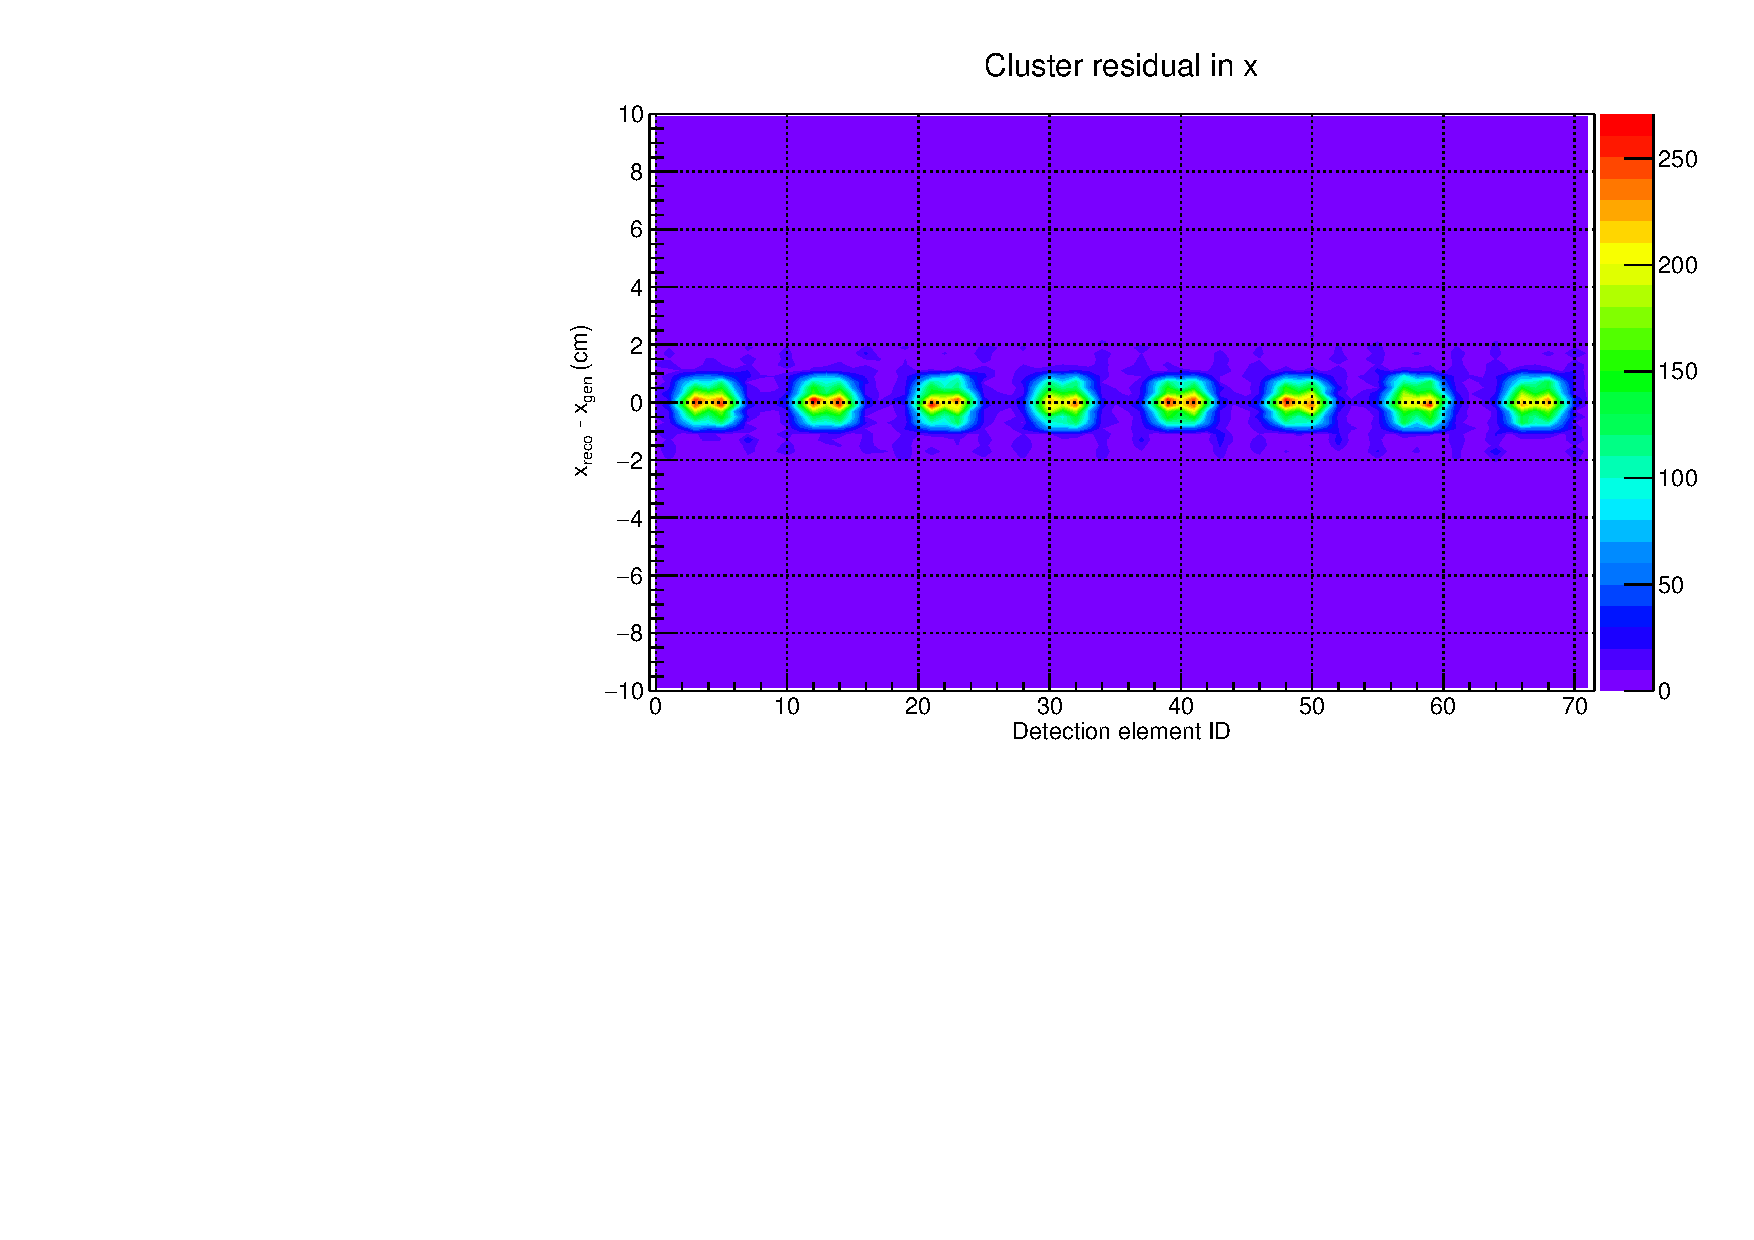
\includegraphics[width=0.9\linewidth]{Chapters/O2/Figs/CRx.pdf}
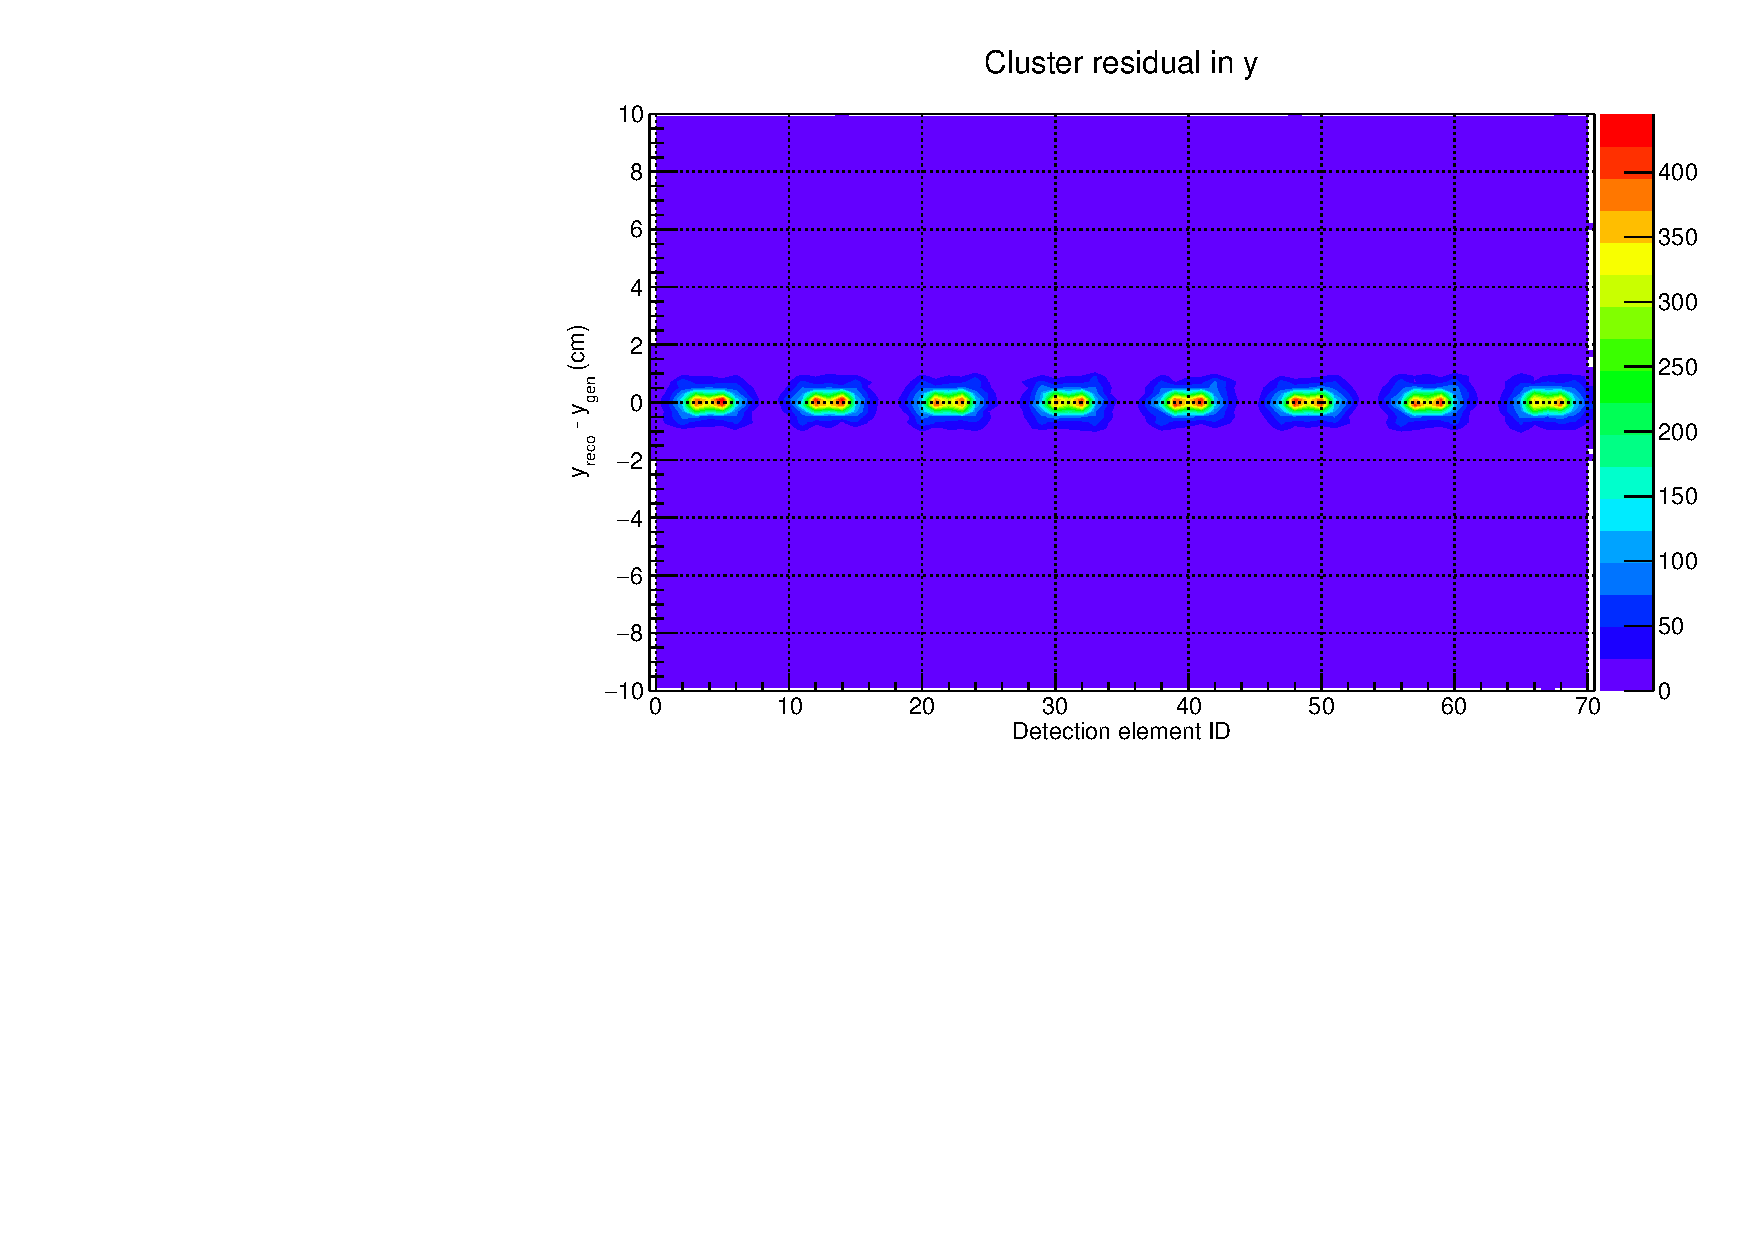
\includegraphics[width=0.9\linewidth]{Chapters/O2/Figs/CRy.pdf}
\caption{Cluster residuals distribution as a function of the RPC ID. The $y$ bins are continuous values, while each $x$ axis bin represents a single RPC. The square shaped artifacts are related to the different strip pitches each RPC is equipped with. The RPCs equipped with strips down to $1$ cm wide present the hot spots due to the superposition of the residuals distributions of $1$, $2$ and $4$ cm wide strips. The $y$ distribution presents smaller structures since the average strip size is smaller. Each RPC distribution is not normalized on its irradiation hence the colour palette is the same for all the RPCs.}
\label{fig:MID_CR}
\end{center}
\end{figure}

\subsection{Track residuals}
Another set of residuals has been computed comparing the generated information to the reconstructed tracks.
In this case all the tracks are described by three spatial coordinates for the crossing point in the first chamber and two deviations, one along $x$, the other along $y$.
The residuals between such parameters have been computed and shown as a function of the position within the RPCs as well as from the kinematic parameters of the track.
This test can be performed using simulated muon tracks for RUN2.

% The test consists in getting a list of reconstructed tracks from RUN2 data.
% The same data file used for the cluster size and cluster residuals evaluation has been processed for this test.
The tracking algorithm is applied to the set of digits and the reconstructed tracks are recorded in the form of a 3D crossing point on the first MID station and a 2D slope.
% Such measurements are compared to the output of the old tracking algorithm.
The residuals distributions of cluster positions and tracks comparison are generated as a function of the detection element (i.e. the RPC) and of the generated total momentum $p$ of the particle.

% The action of the Kalman filter is the reduction of the effect of the spatial segmentation typical of a stripped/padded detector.
% For this reason the tracks residuals are less affected by the strips size.
% The residuals are shown as a function of the reconstructed momentum $p$ of the particles.
The spatial resolution along $x$ and $y$ are shown in figures \ref{fig:MID_xpoint_x} and \ref{fig:MID_xpoint_y} respectively, as a function of the generated total momentum of the particle.
The residuals normalized on the residual uncertainty are shown in figure \ref{fig:MID_TRm}.
Most of the measurements are within 3 sigmas as expected, except for extremely low momenta particles.
The distribution gets narrower moving to higher $p$ particles.
It is worth noting that the binning of the histogram varies versus $p$, in particular going from $1\ GeV/c$ to $2\ GeV/c$ for $p\ =\ 20 GeV/c$.
Both distributions are centered at $0$ cm.
As expected, considering the detector morphology, the vertical resolution ($0.4$ cm) is better than the horizontal one ($0.7$ cm).
% The distributions relative to the crossing point are reported in figures \ref{fig:MID_xpoint_x} and \ref{fig:MID_xpoint_y}.
The spatial resolutions are reflected in the slope resolutions.
In order to better understand the angular resolution, the distribution is shown as the residual divided by the uncertainty that is automatically calculated by the Kalman filter.
Up to the $95\%$ of the distribution is within the $\pm1.96$ band in the vertical slope distribution.
The distribution gets physiologically broader at lower $p_\mathrm{T}$.

\begin{figure}[!ht]
\begin{center}
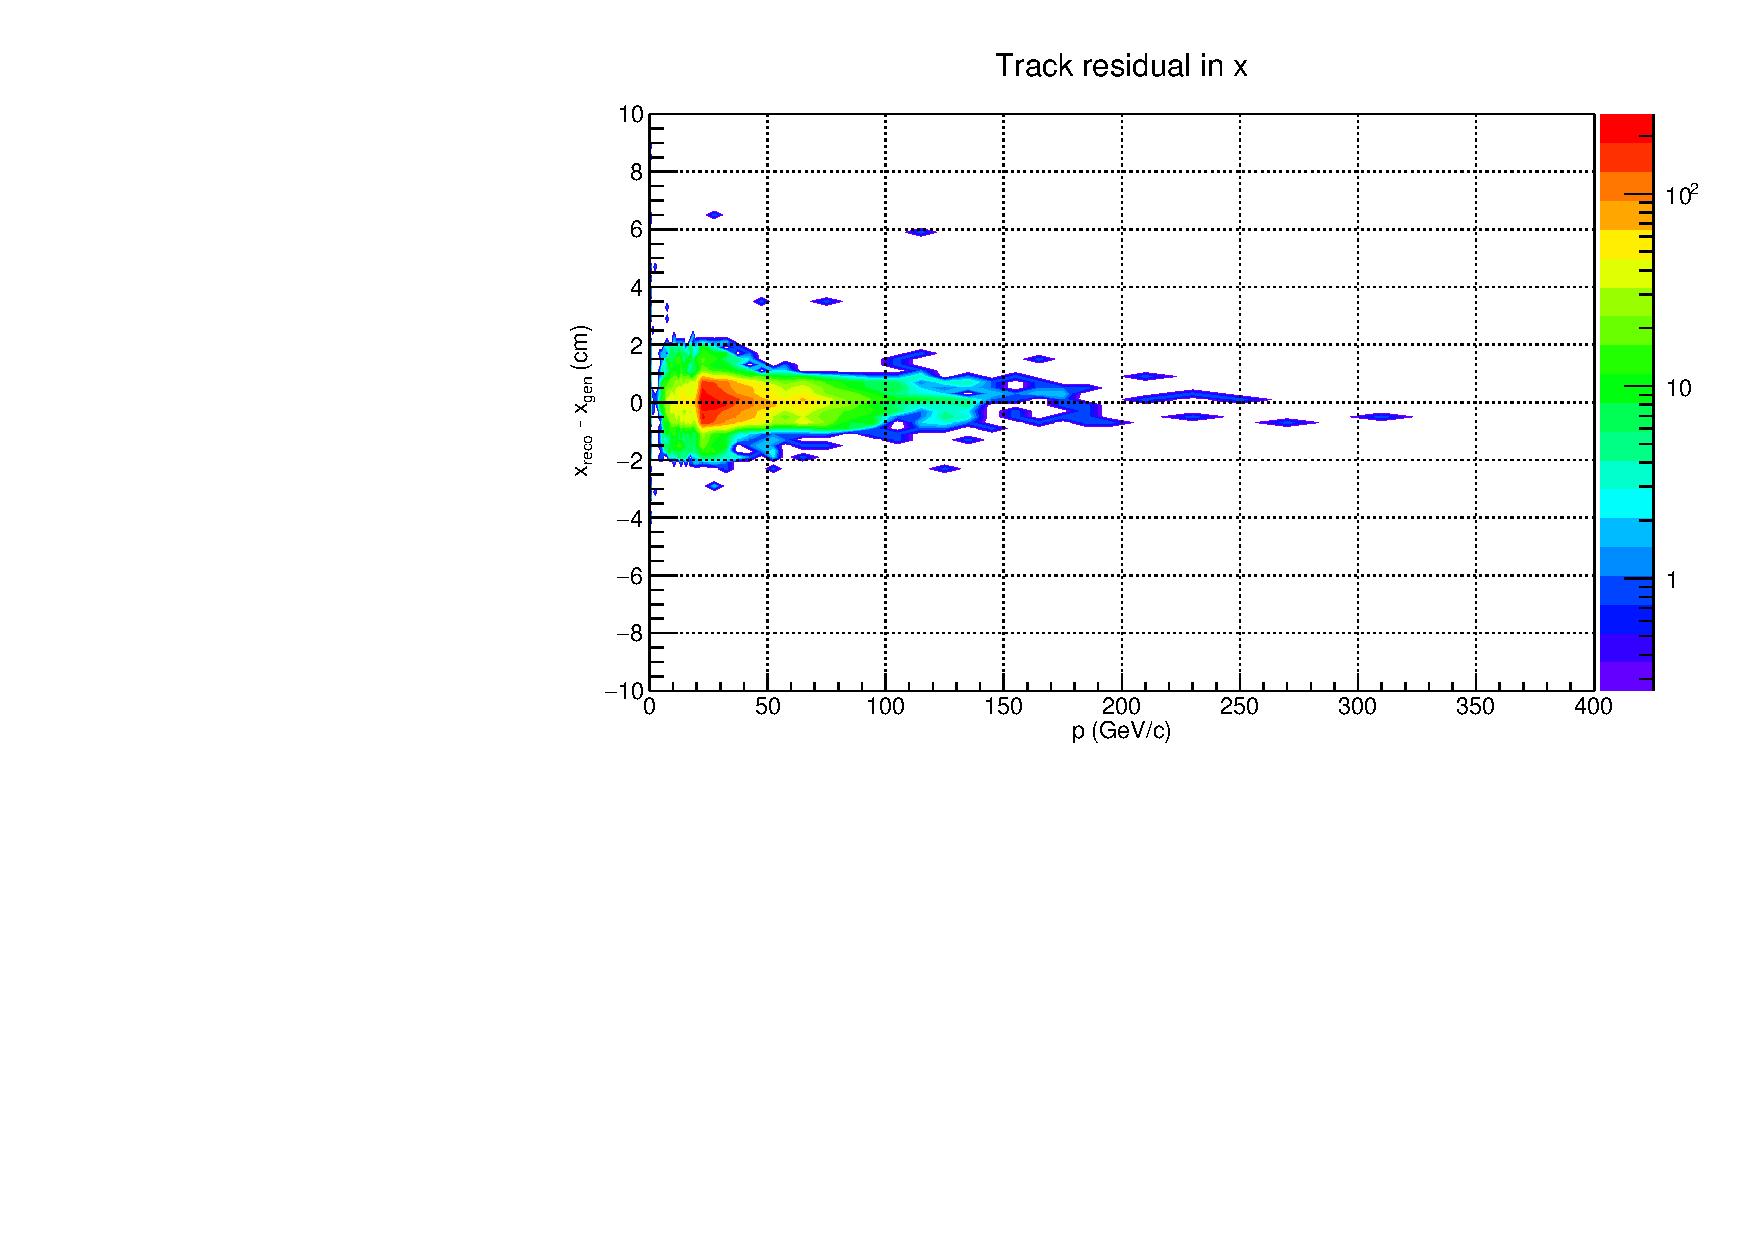
\includegraphics[width=0.99\linewidth]{Chapters/O2/Figs/TRx.pdf}
\caption{Track residuals distribution of the horizontal coordinate. The $y$ axis represents the residual expressed in centimeters, while the $x$ axis is the generated momentum of the particle. The colour palette is in logarithmic scale.
The core of the distribution is about $1$ cm wide and very few outliers cross the $\pm2$ cm band.}
\label{fig:MID_xpoint_x}
\end{center}
\end{figure}

\begin{figure}[!ht]
\begin{center}
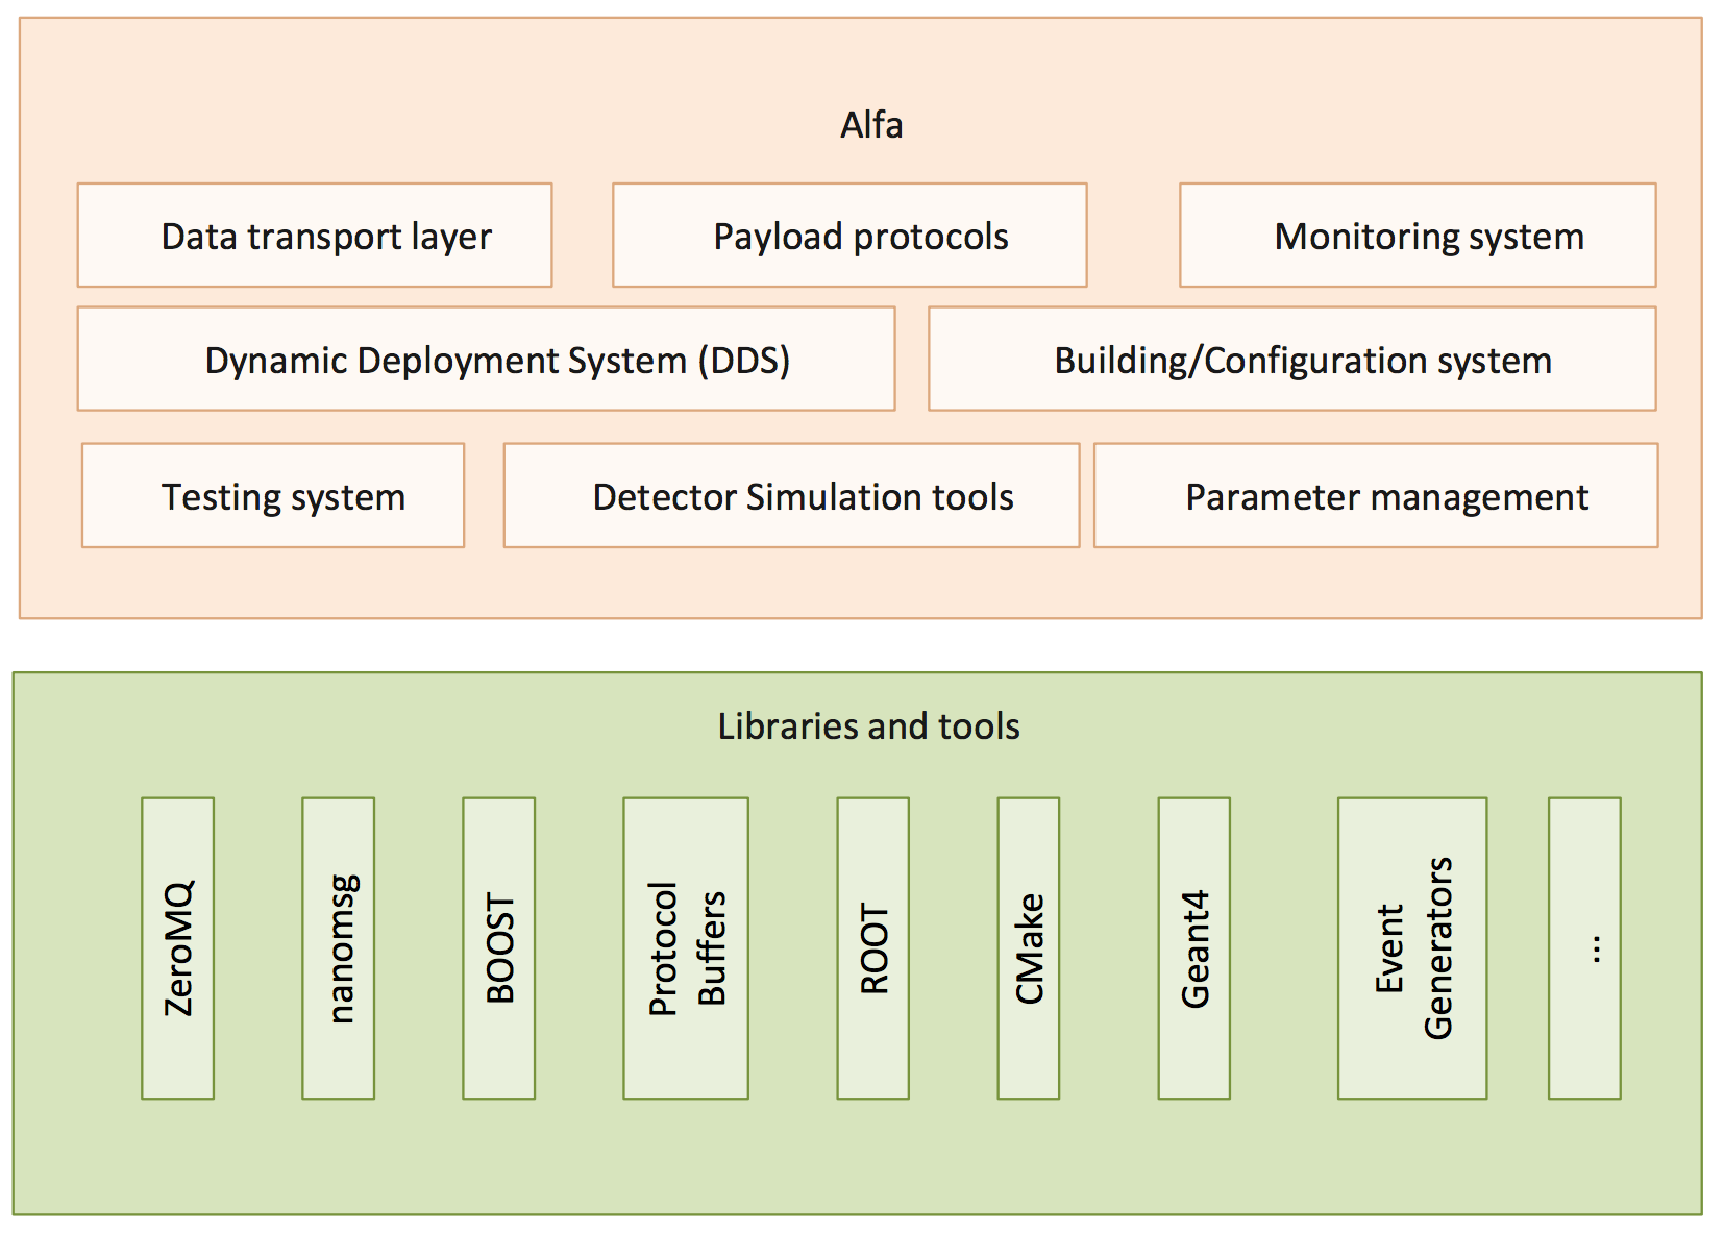
\includegraphics[width=0.99\linewidth]{Chapters/O2/Figs/TRy.pdf}
\caption{Track residuals distribution of the vertical coordinate. The $y$ axis represents the residual expressed in centimeters, while the $x$ axis is the reconstructed momentum of the particle. The colour palette is in logarithmic scale.
The core of the distribution is about $0.5$ cm wide and like for the horizontal coordinate, very few outliers cross the $\pm2$ cm band.}
\label{fig:MID_xpoint_y}
\end{center}
\end{figure}

\begin{figure}[!h]
\begin{center}
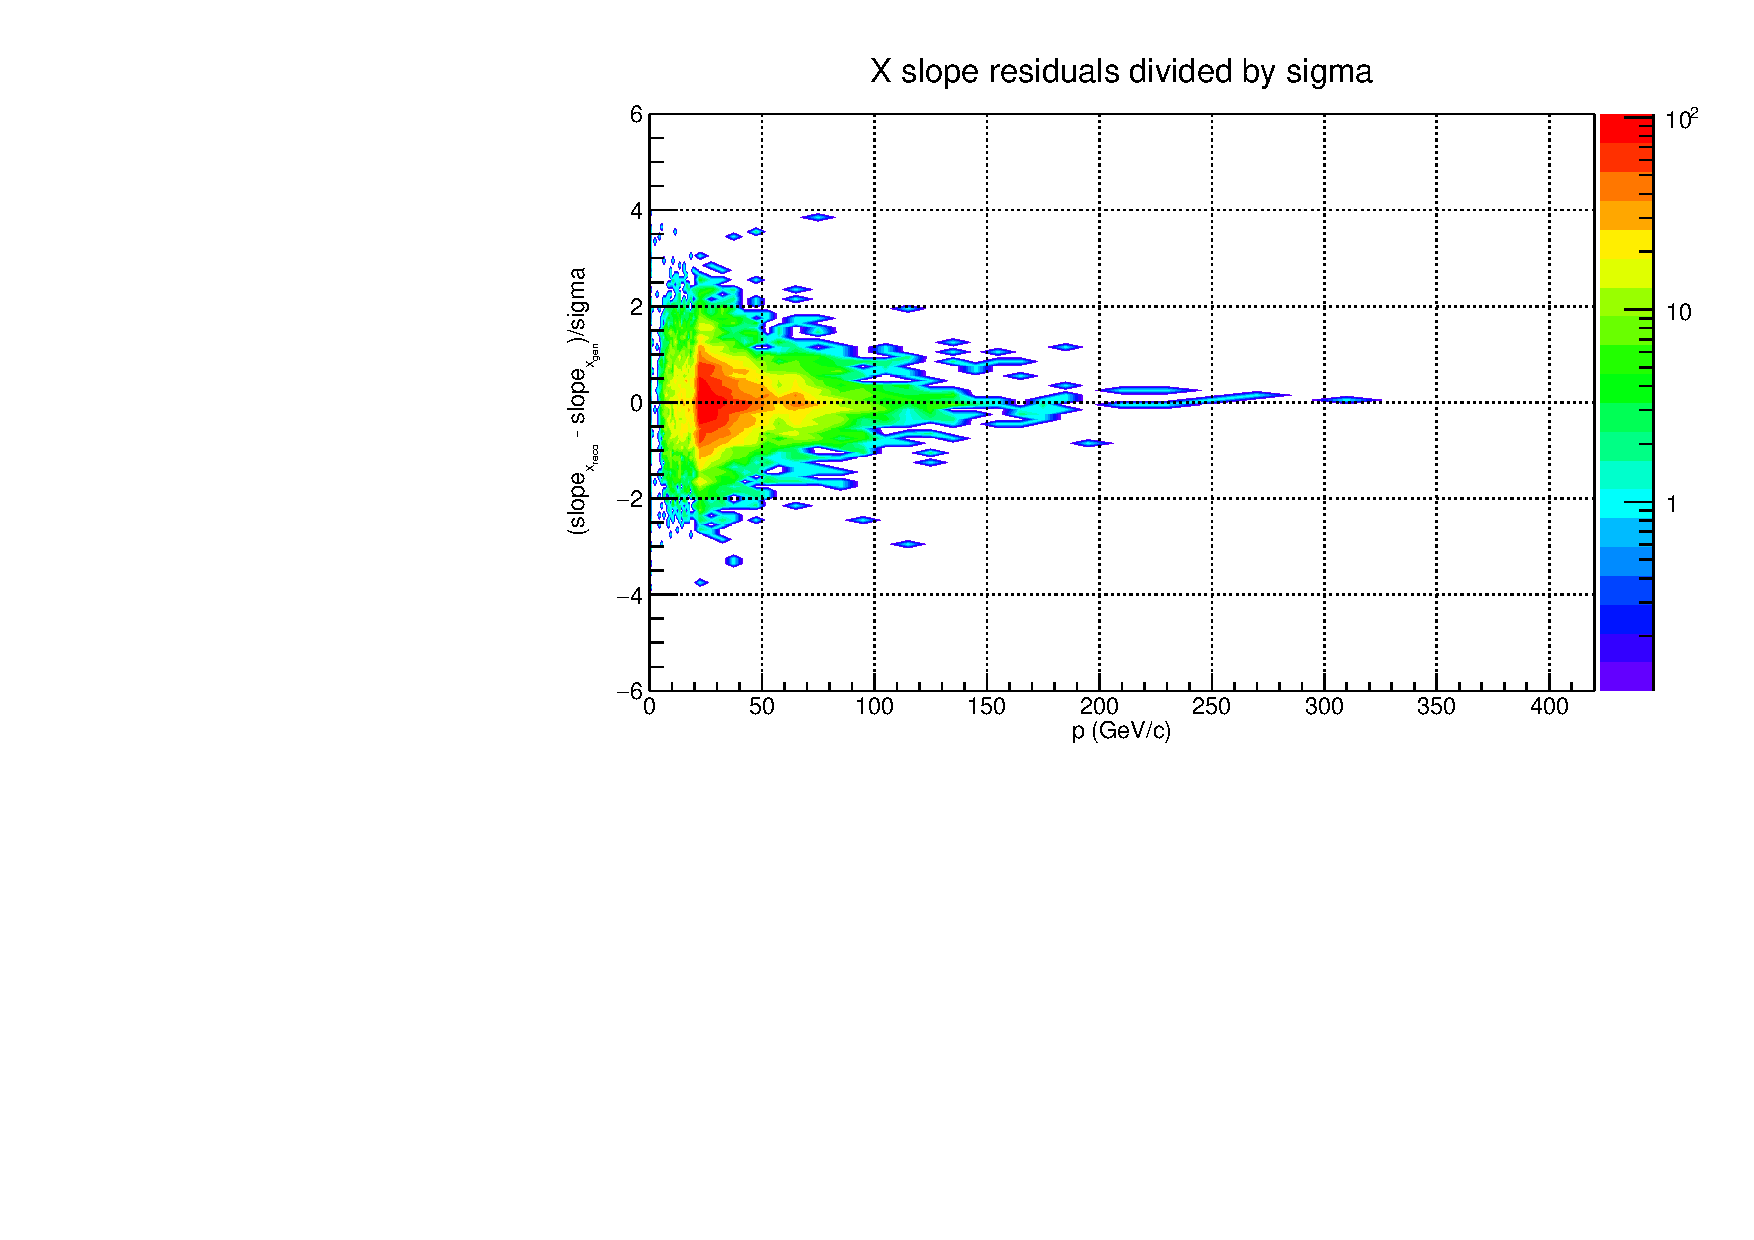
\includegraphics[width=0.99\linewidth]{Chapters/O2/Figs/TRmx_sigma.pdf}
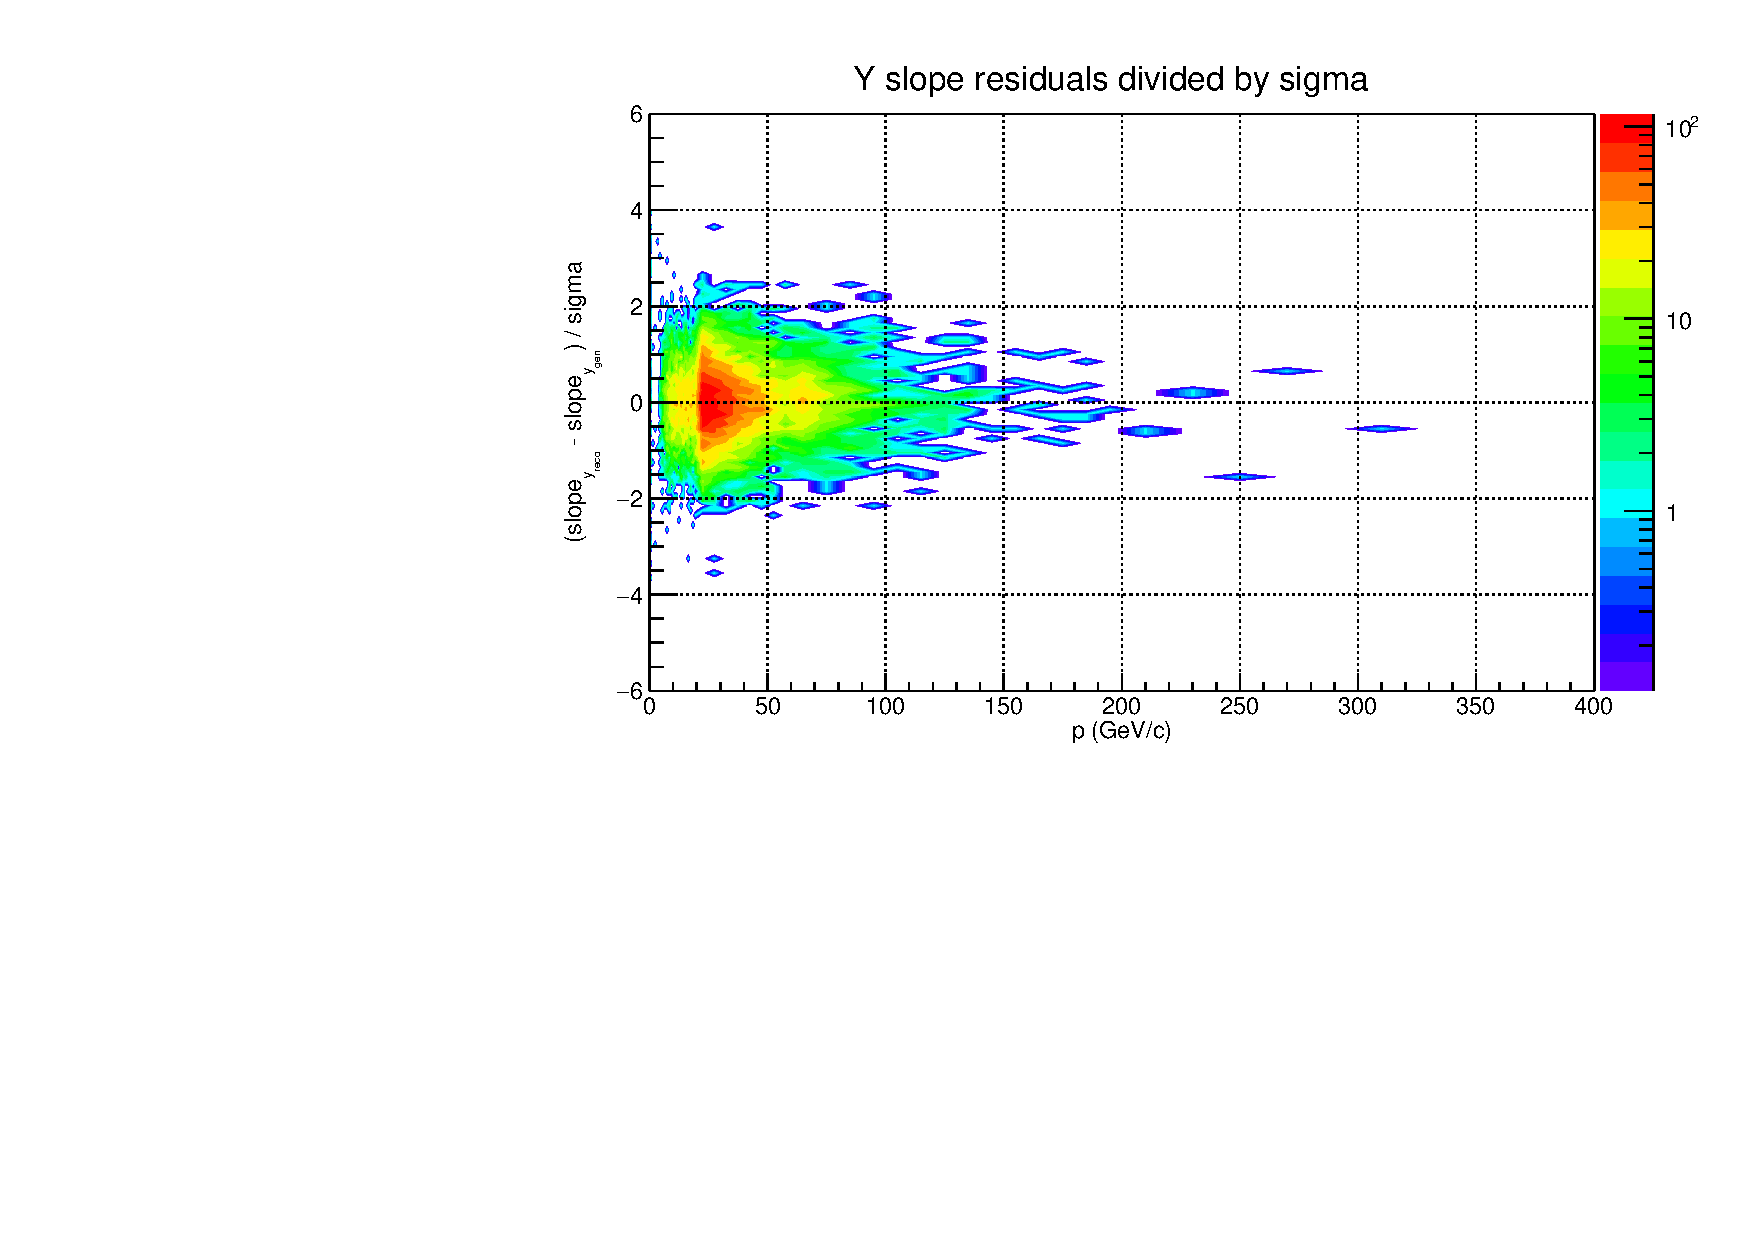
\includegraphics[width=0.99\linewidth]{Chapters/O2/Figs/TRmy_sigma.pdf}
\caption{Residuals of the vertical and horizontal slopes evaluation between the old MTR's algorithm and the new MID's one. The values are represented as residuals ($y$) divided by sigma as a function of the reconstructed particle momentum. The colour pallette is represented in logarithmic scale.}
\label{fig:MID_TRm}
\end{center}
\end{figure}

The overall resolution presents a clear dependence with respect to the particle momentum.
A lower resolution has been measured for low impulse particles, while the distribution spread decreases moving to higher momentum.
The fine tuning of the algorithm has not yet been performed and such optimization could help solving the issue.

% \subsection{Algorithm resolution}
% The residuals computed between two outputs are equivalent to the resolution plots of one of the two methods if and only if the other algorithm is the perfect or ideal one.
% Since the MTR algorithm was not ideal, the comparison reported in the previous section is not equivalent to a resolution measurement.

% A proper way to determine the reconstruction resolution of a given algorithm is to use as input and control variables the information generated by a simulation whose Monte Carlo truth is accessible.
% The reconstruction algorithm is applied to the simulated data and its output is recorded.
% Since using a Monte Carlo simulation allows one to access the true particle parameters, the residuals are computed between such parameters and the reconstructed tracks' ones.

% The residuals distributions features, such as the mean values and the standard deviation, can be used to evaluate possible algorithmic biases leading to a polarized residuals distribution and, in general, to associate an error to the reconstructed parameters.

% The Monte Carlo simulation used for such tests should emulate the tracks multiplicity expected in the real events.
% In fact, the overlapping of clusters belonging to different particles might lead to worse performances caused by bad clusters selection or centroid computation.
% This benchmark has not yet been performed and is expected as future development.

\subsection{Tracking efficiency}
The measurement of the algorithm resolution is not the only crucial test for a new tracking method.
An algorithm might present exceptional resolution on a negligible fraction of the processed tracks.
For this reason the evaluation of the tracking efficiency, defined as the ratio between processed particles and reconstructed ones, is crucial.
% The study of the reconstruction efficiency can be performed using Monte Carlo simulations as input.
% The simulations which can be used for such study are either full simulations or embedded simulations.
% While the full simulations are events completely simulated using a generator, the embedded simulations are real events which are provided with an overlapped simulation of a specific signal.
% In this case the embedded simulations are created generating a quarkonium state forced to decay in an unlike sign muon pair within the MID acceptance.
% The efficiency of the reconstruction is the ratio between the number of reconstructed and generated muons.
% The quarkonia states reconstruction efficiency is the product of the reconstruction efficiencies of the two muons.
% It is important to evaluate the differential reconstruction efficiency with respect to cinematic variables such as rapidity and (transverse) momentum.
The tracking efficiency was estimated using the same MC as the one used for the residuals. 
The results of this study are reported in figure \ref{fig:ID_eff}.
The measured efficiency is very close to unity.
Some bins at the edge of the muon spectrometer $p_{\mathrm{T}}$ and $y$ acceptance, show an efficiency drop\footnote{Entries at zero efficiency mostly correspond to $p_{\mathrm{T}}$ and $y$ bins where no generated muon fell in.}.
The study should be repeated in the future with simulations embedded in real events in order to assess the efficiency of the algorithm at high particle multiplicity.

\begin{figure}[!b]
\begin{center}
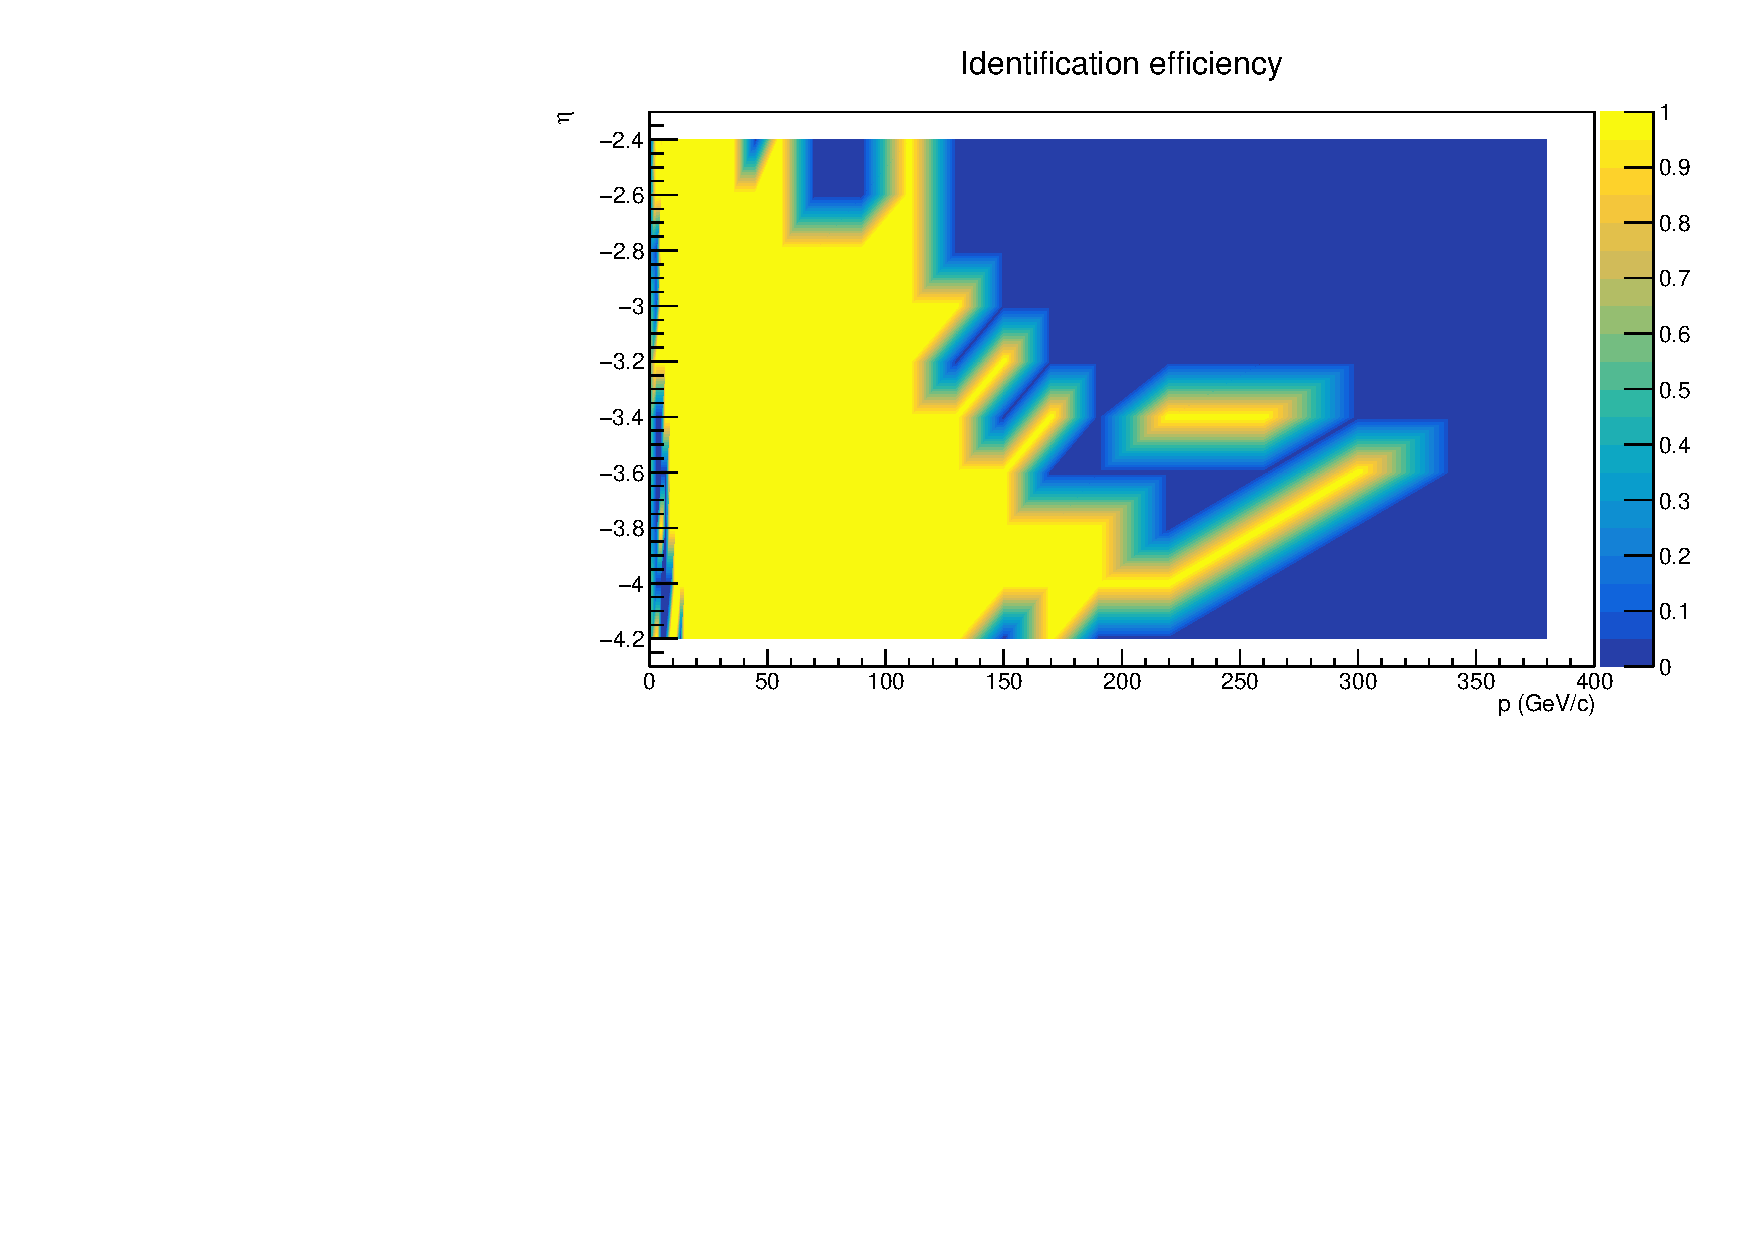
\includegraphics[width=0.9\linewidth]{Chapters/O2/Figs/ID_Eff.pdf}
\caption{Tracking efficiency computed as the ratio between the numbers of reconstructed and generated tracks.}
\label{fig:ID_eff}
\end{center}
\end{figure}

\subsection{PID characterization}
The PID performance of the new algorithm has to be evaluated.

First of all the PID efficiency has to be computed.
This characteristic of the algorithm corresponds to its matching probability.
Such measurement can be performed evaluating how many real muons are matched with muon tracker data, hence correctly flagged.
Using Monte Carlo simulations one can measure such fraction computing the ratio between reconstructed muons and reconstruct-able muons.
A reconstruct-able muon is a muon which has been generated within the muon spectrometer acceptance and left hits in both MCH and MID.

Secondly the fraction of mis-identified particles should be computed as well.
Some particles which are not muons are detected and reconstructed in the MCH.
If they get matched with some MID tracklets then become wrongly flagged as muons.
In order to evaluate this mis-identification probability one should compute the ratio between the number of non-muons matched in the MID and the number of non-muons reconstructed in the MCH.

Both these characterizations have not been performed yet.

% The mis-identification probability is then evaluated using complete Monte Carlo simulations, in order to be able to know the real identity of each identified particle.
% The probability of mis-identification is then evaluated as the ratio between the number of non-muons identified as such divided by the total number of identified particles.
% Given a particle has been tagged as muon, the mis-identification probability corresponds to the inverse of the significance of the identification itself.
% The density of non muons reaching the MID is higher closer to the beam pipe, at high rapidities.
% For this reason the differential study is necessary to be sure that the mis-identification probability is low at least in the lowest rapidity region to limit as much as possible the pollution from other particles.
% Such measurement has not been performed yet.